% Options for packages loaded elsewhere
\PassOptionsToPackage{unicode}{hyperref}
\PassOptionsToPackage{hyphens}{url}
%
\documentclass[
]{book}
\usepackage{amsmath,amssymb}
\usepackage{lmodern}
\usepackage{iftex}
\ifPDFTeX
  \usepackage[T1]{fontenc}
  \usepackage[utf8]{inputenc}
  \usepackage{textcomp} % provide euro and other symbols
\else % if luatex or xetex
  \usepackage{unicode-math}
  \defaultfontfeatures{Scale=MatchLowercase}
  \defaultfontfeatures[\rmfamily]{Ligatures=TeX,Scale=1}
  \setmainfont[]{Libre Baskerville}
\fi
% Use upquote if available, for straight quotes in verbatim environments
\IfFileExists{upquote.sty}{\usepackage{upquote}}{}
\IfFileExists{microtype.sty}{% use microtype if available
  \usepackage[]{microtype}
  \UseMicrotypeSet[protrusion]{basicmath} % disable protrusion for tt fonts
}{}
\makeatletter
\@ifundefined{KOMAClassName}{% if non-KOMA class
  \IfFileExists{parskip.sty}{%
    \usepackage{parskip}
  }{% else
    \setlength{\parindent}{0pt}
    \setlength{\parskip}{6pt plus 2pt minus 1pt}}
}{% if KOMA class
  \KOMAoptions{parskip=half}}
\makeatother
\usepackage{xcolor}
\usepackage[left=4cm, right=3cm, top=2.5cm, bottom=2.5cm]{geometry}
\usepackage{listings}
\newcommand{\passthrough}[1]{#1}
\lstset{defaultdialect=[5.3]Lua}
\lstset{defaultdialect=[x86masm]Assembler}
\usepackage{longtable,booktabs,array}
\usepackage{calc} % for calculating minipage widths
% Correct order of tables after \paragraph or \subparagraph
\usepackage{etoolbox}
\makeatletter
\patchcmd\longtable{\par}{\if@noskipsec\mbox{}\fi\par}{}{}
\makeatother
% Allow footnotes in longtable head/foot
\IfFileExists{footnotehyper.sty}{\usepackage{footnotehyper}}{\usepackage{footnote}}
\makesavenoteenv{longtable}
\usepackage{graphicx}
\makeatletter
\def\maxwidth{\ifdim\Gin@nat@width>\linewidth\linewidth\else\Gin@nat@width\fi}
\def\maxheight{\ifdim\Gin@nat@height>\textheight\textheight\else\Gin@nat@height\fi}
\makeatother
% Scale images if necessary, so that they will not overflow the page
% margins by default, and it is still possible to overwrite the defaults
% using explicit options in \includegraphics[width, height, ...]{}
\setkeys{Gin}{width=\maxwidth,height=\maxheight,keepaspectratio}
% Set default figure placement to htbp
\makeatletter
\def\fps@figure{htbp}
\makeatother
\setlength{\emergencystretch}{3em} % prevent overfull lines
\providecommand{\tightlist}{%
  \setlength{\itemsep}{0pt}\setlength{\parskip}{0pt}}
\setcounter{secnumdepth}{5}
\newlength{\cslhangindent}
\setlength{\cslhangindent}{1.5em}
\newlength{\csllabelwidth}
\setlength{\csllabelwidth}{3em}
\newlength{\cslentryspacingunit} % times entry-spacing
\setlength{\cslentryspacingunit}{\parskip}
\newenvironment{CSLReferences}[2] % #1 hanging-ident, #2 entry spacing
 {% don't indent paragraphs
  \setlength{\parindent}{0pt}
  % turn on hanging indent if param 1 is 1
  \ifodd #1
  \let\oldpar\par
  \def\par{\hangindent=\cslhangindent\oldpar}
  \fi
  % set entry spacing
  \setlength{\parskip}{#2\cslentryspacingunit}
 }%
 {}
\usepackage{calc}
\newcommand{\CSLBlock}[1]{#1\hfill\break}
\newcommand{\CSLLeftMargin}[1]{\parbox[t]{\csllabelwidth}{#1}}
\newcommand{\CSLRightInline}[1]{\parbox[t]{\linewidth - \csllabelwidth}{#1}\break}
\newcommand{\CSLIndent}[1]{\hspace{\cslhangindent}#1}
\usepackage{float}
\floatplacement{figure}{H}
\usepackage{booktabs}
\usepackage{setspace}
\usepackage{fontspec}
\onehalfspacing
\usepackage{xcolor}
\usepackage{titlesec}
\usepackage{xfrac}
% Make caption labels bold: https://bookdown.org/yihui/rmarkdown-cookbook/latex-extra.html
\usepackage[labelfont={bf}]{caption} 
% force floats forward: https://bookdown.org/yihui/rmarkdown-cookbook/figure-placement.html
\usepackage{flafter}
% https://tex.stackexchange.com/questions/279/how-do-i-ensure-that-figures-appear-in-the-section-theyre-associated-with
\usepackage{placeins}
\lstset{
  breaklines=true
}
\usepackage{wrapfig}
\usepackage{lipsum}
\usepackage{caption}
\captionsetup[figure]{font=small}
% following code copied from https://bookdown.org/yihui/rmarkdown-cookbook/figure-placement.html#fnref10 
\renewcommand{\topfraction}{.85}
\renewcommand{\bottomfraction}{.7}
\renewcommand{\textfraction}{.15}
\renewcommand{\floatpagefraction}{.66}
\setcounter{topnumber}{3}
\setcounter{bottomnumber}{3}
\setcounter{totalnumber}{4}

%% https://stackoverflow.com/questions/3275770/modifying-section-to-make-it-colorful-with-latex
%\usepackage{color}
%\titleformat{\section}
%{\color{red}}


% https://tex.stackexchange.com/questions/10320/section-and-subsection-colors-using-titlesec
%\makeatletter
%\newcommand*\@secondofsix[6]{#2}
%\newcommand{\addtotitleformat}{%
%  \@ifstar{\addtotitleformat@star}{\addtotitleformat@nostar}}
%\newcommand\addtotitleformat@nostar[2]{%
%  \PackageError{titlesec}{non starred form of \string\addtotitleformat\space not supported}{}}
%\newcommand\addtotitleformat@star[2]{%
%  \expandafter\expandafter\expandafter\expandafter
%  \expandafter\expandafter\expandafter\def
%  \expandafter\expandafter\expandafter\expandafter
%  \expandafter\expandafter\expandafter\@currentsection@font
%  \expandafter\expandafter\expandafter\expandafter
%  \expandafter\expandafter\expandafter{%
%    \expandafter\expandafter\expandafter\@secondofsix
%       \csname ttlf@\expandafter\@gobble\string#1\endcsname}%
%  \titleformat*{#1}{\@currentsection@font#2}%
%}
%\makeatother
%
%\addtotitleformat*{\section}{\Huge\color{red}}
%\addtotitleformat*{\subsection}{\sffamily\color{blue}}
\usepackage{titling}
\usepackage{subcaption}
\pretitle{\begin{center} 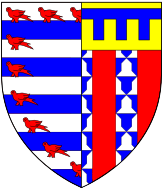
\includegraphics[width=2in,height=2in]{/Users/brettell/Documents/Repositories/PhD-thesis/book/figs/title/Arms_PembrokeCollege_Cambridge.pdf}\LARGE\\ \bigskip \bigskip \bigskip }
\posttitle{\end{center}}
\predate{\begin{center} Pembroke College \\ \bigskip }
\postdate{\end{center} \begin{center} \bigskip \bigskip \bigskip This thesis is submitted for the degree of Doctor of Philosophy. \end{center} \centering \begin{figure}[!tpb] \centering \begin{subfigure}{0.49 \linewidth} \centering \vfill \includegraphics[height=0.45in]{/Users/brettell/Documents/Repositories/PhD-thesis/book/figs/title/cambridge_university2.pdf} \end{subfigure} \hfill \begin{subfigure}{0.49 \linewidth} \centering \includegraphics[height=0.55in]{/Users/brettell/Documents/Repositories/PhD-thesis/book/figs/title/EMBL_EBI_Logo_black.pdf} \end{subfigure} \end{figure} }
\usepackage{float}
\ifLuaTeX
  \usepackage{selnolig}  % disable illegal ligatures
\fi
\IfFileExists{bookmark.sty}{\usepackage{bookmark}}{\usepackage{hyperref}}
\IfFileExists{xurl.sty}{\usepackage{xurl}}{} % add URL line breaks if available
\urlstyle{same} % disable monospaced font for URLs
\hypersetup{
  pdftitle={Japanese courage: a genetic analysis of complex traits in medaka fish and humans},
  pdfauthor={Ian Narain Brettell},
  hidelinks,
  pdfcreator={LaTeX via pandoc}}

\title{Japanese courage: a genetic analysis of complex traits in medaka fish and humans}
\author{Ian Narain Brettell}
\date{30 September 2022}

\begin{document}
\maketitle

{
\setcounter{tocdepth}{1}
\tableofcontents
}
\hypertarget{acknowledgements}{%
\chapter*{Acknowledgements}\label{acknowledgements}}
\addcontentsline{toc}{chapter}{Acknowledgements}

Thanks.

\hypertarget{preface}{%
\chapter*{Preface}\label{preface}}
\addcontentsline{toc}{chapter}{Preface}

This thesis is the result of my own work and includes nothing which is the outcome of work done in collaboration except as declared in the preface and specified in the text.

It is not substantially the same as any work that has already been submitted before for any degree or other qualification except as declared in the preface and specified in the text.

It does not exceed the prescribed word limit for the Degree Committee for the Faculty of Biology.

\hypertarget{abstract}{%
\chapter*{Abstract}\label{abstract}}
\addcontentsline{toc}{chapter}{Abstract}

This thesis primarily explores how an individual's genes interact with the genes of their social companions to create differences in behaviour, using the Japanese medaka fish as a model organism. Chapter 1 sets out the introduction to the diverse topics covered in this thesis.

Chapter 2 describes several genomic characteristics of the Medaka Inbred Kiyosu-Karlsruhe (MIKK) panel, which comprises 80 inbred lines of medaka that were bred from a wild population found in the city of Kiyosu, in southern Japan. In this chapter I plot the inbreeding trajectory of the MIKK panel and analyse a number of genomic characteristics relevant to its utility for the genetic mapping of complex traits, including: the panel's evolutionary relationship with other previously established inbred medaka strains; the degree of homozygosity in the inbred lines; the rate of linkage disequilibrium decay across the panel; and the genomic repeats and structural variation present in their genomes.

In Chapter 3, I use a custom behavioural assay to characterise and classify bold-shy behaviours in 5 previously established inbred medaka lines. I describe the assay, assess its robustness against confounding factors, and apply a hidden markov model (HMM) to classify the fishes' behaviours across a spectrum of boldness-shyness based on the individuals' distance and angle of travel between pre-defined time intervals. I describe how the lines differ in their behaviours over the course of the assay (a ``direct genetic effect'') and how the behaviour of a single ``reference'' line (\emph{iCab}) differs in the presence of different lines (a ``social genetic effect'').

In Chapter 4 I describe the bioinformatic processes and genetic association models that I used to map the variants associated with differences in the period of somite development, based on an F2 cross between the southern Japanese \emph{iCab} strain, and the northern Japanese \emph{Kaga} strain.

In Chapter 5, I explain how I ran our custom behavioural assay over the MIKK panel to identify lines that diverge in both their own bold-shy behaviours (the direct genetic effect) and the extent to which they transmit those behaviours onto their tank partners (the social genetic effect). I then describe how I used those divergent lines as the parental lines in a multi-way F2 cross in an attempt to isolate the genetic variants that are associated with both direct and social genetic effects.

Finally, in Chapter 6, I turn to humans to compare and rank all complex traits in the GWAS Catalog based on the extent to which their associated alleles vary across global populations, using the Fixation Index (\(F_{ST}\)) as a metric, and the 1000 Genomes dataset as a sample of global genetic variation. In this chapter I set out the bioinformatic pipelines used to process the data, present the distributions of \(F_{ST}\) for trait-associated alleles across the genome, and use the Kolmogorov-Smirnov test to compare the distributions of \(F_{ST}\) across different traits.

Altogether, this thesis describes some of the genomic characteristics of both medaka fish and humans, and how those variations relate to differences in complex traits, with a particular focus on the genetic causes of adaptive behaviours and the transmission of those behaviours onto one's social companions.

\hypertarget{Introduction}{%
\chapter{Introduction}\label{Introduction}}

Humankind has long sought to understand the basis of biological variation. What gives rise to the wondrous variety of life forms on Earth? Why do individuals of a particular species differ from one another? How do children inherit traits that are similar to those of their parents, yet on the whole remain distinct from both their parents and their siblings? And are the traits we care about -- our health, our BEHAVIOUR {[}NEED TO GET THE SOCIAL ENVRIONMENT OUT{]} intelligence, our ability to thrive in a changing world -- pre-determined from birth, or continuously pliable throughout our lives? These questions fundamentally concern the natural laws of inheritance, which until recently remained mysterious and obscure. Rapidly-improving technologies are making these questions increasingly tractable, yet the interplay between genes and environment are still the subject of controversy, especially in relation to human traits such as intelligence.

In this thesis, I primarily explore the extent to which phenotypic variation is determined by an individual's own genes, and how much it is mediated by the genes of one's social companions, with a particular focus on the phenotype of bold-type behaviours in the Japanese rice paddy fish \emph{Oryzias latipes}. I first provide a brief history of the field, describing some of the work of the scientists on whose shoulders this research stands, from Charles Darwin's theory of evolution, Mendel's identification of the units of inheritance, and the study of continuous variation by Francis Galton, Karl Pearson, Ronald Fisher, and Sewall Wright, but also touching on their other legacies.{[}BRING EUGENICS INTO MAIN TEXT.{]} I then outline the traditional animal crossing methods and modern DNA sequencing and statistical techniques that I used to parse the respective contributions of genes and environment to variation in complex traits, and ultimately identify the genetic variants that drive those differences. {[}I'M ALSO GOING TO GIVE YOU AN INTRODUCTION THTE PHENOTYPES I STUDY IN MEDAKA{]}

\hypertarget{a-brief-history-of-genetics}{%
\section{A brief history of genetics}\label{a-brief-history-of-genetics}}

Much of this section has been informed by Mukherjee (2016), Rutherford (2020), and Tabery (2014). Where possible, I have cited the original sources.

\hypertarget{ancient-greece}{%
\subsection{Ancient Greece}\label{ancient-greece}}

Throughout ancient history, the sources of biological variation were completely unknown. With limited technologies available to them, the Ancient Greek philosophers proposed theories for the inheritance of traits that they observed in humans. Around 500 BC, Pythagoras applied his knowledge of triangles to the question of how traits are inherited from one's parents. He proposed the theory known as ``spermism'', positing that hereditary information was passed down from parent to child via male sperm, with the female providing the nutrients that would allow it to grow. Like the theorem that bears his name, he supposed that these two sides of the ``triangle'' would determine the length of the third side: the characteristics of the child (Mukherjee 2016). Over a century later, in 380 BC, Plato extended this metaphor in \emph{The Republic} (Badiou 2013) to argue that this principle could be applied to perfect humanity by breeding perfect combinations of parents at perfect times (Mukherjee 2016), which is possibly the first recorded expression of eugenic intent.

Aristotle later joined the discussion with his treatise \emph{Generation of Animals} (Aristotle 2021), where he noted that children inherited features from their mothers as well as their fathers, raising cases where human skin colour and other traits from maternal ancestors could skip generations, and thus sperm could not be the only vessel of hereditary information. He suggested an idea of ``movement'' -- the transmission of information -- from the father's sperm, which sculpts the mother's menstrual blood in the same way a carpenter carves a piece of wood. It was, however, impossible for Aristotle to deduce the form in which the information was conveyed.

\hypertarget{middle-ages}{%
\subsection{Middle Ages}\label{middle-ages}}

From medieval times through to the 1800s, the prevailing theory of heredity was that a tiny human -- a homunculus -- sat within the sperm, waiting to be inflated upon its introduction to a woman's uterus. But from where did each previous homunculus originate? Logically, the theory would require each homunculus to hold another homunculus, \emph{ad infinitum}. This theory deceived the inventor of the microscope, Nicolaas Hartsoeker, into thinking he observed a homunculus in a sperm he was studying (\textbf{Figure \ref{fig:homunculus-pic}}) (Hartsoeker 1694). But a fundamental question remained: what triggered the expansion of the human form, causing the embryo to develop new parts on its road to becoming a fetus? The answer could only have been some instruction, blueprint, or code, but any specifics remained out of reach.



\begin{figure}

{\centering \includegraphics[width=0.5\linewidth]{figs/introduction/homunculus} 

}

\caption{Preformation, drawn by Nicolaas Hartsoeker in 1695. Image adapted from Commons (2019).}\label{fig:homunculus-pic}
\end{figure}

\hypertarget{charles-darwin}{%
\subsection{Charles Darwin}\label{charles-darwin}}

During the early 1800s, the prevailing doctrine on the origins of biological variation was Creationism, based on Christianity's literal interpretation of the Bible's Book of Genesis (Campbell 2010). Any mechanistic description of how species -- and individuals within the same species -- differed from one another was thought to threaten this doctrine, making inquiries of this kind potentially blasphemous, and therefore dangerous (Armstrong 2000).

It was in this context that a 22-year-old English clergyman named Charles Darwin (\textbf{Figure \ref{fig:charles-darwin-young-portrait}}) boarded the \emph{HMS Beagle} in 1831 to commence a voyage around the world that would last for almost five years (Darwin 2019). Darwin had previously studied theology at the University of Cambridge, but was drawn to study the natural world. He had apprenticed with his fellow clergyman John Henslow, a botanist and geologist who curated the Cambridge Botanic Garden (Isely 2002), who suggested that he join the \emph{Beagle}'s exploratory survey of South America as the ``gentleman scientist'' they were seeking to assist with the collection of specimens (Henslow 1831).



\begin{figure}

{\centering \includegraphics[width=0.7\linewidth]{figs/introduction/Charles_Darwin_by_G._Richmond} 

}

\caption{Portrait of Charles Darwin from the late 1830s by George Richmond (Commons 2017b).}\label{fig:charles-darwin-young-portrait}
\end{figure}

After rounding Cape Horn and moving northward along the western coast of South America, the \emph{HMS Beagle} eventually reached the Galápagos Islands on the coast of Peru, an archipelago of 18 islands formed from volcanic lava (Darwin 1998). Over the course of five weeks, Darwin collected carcasses of birds, lizards, and plants. Upon his return to England, he was hailed as a minor celebrity among natural historians due to the collections of specimens he had gathered and shipped back. John Gould -- the ornithologist who lent his (wife's) name to the Gouldian finch (\textbf{Figure \ref{fig:gouldian-finch}}) -- told him that the various birds that Darwin thought were a variety of wrens, warblers, blackbirds, and ``gros-beaks'' were in fact all 13 different species of finches.



\begin{figure}

{\centering \includegraphics[width=1\linewidth]{figs/introduction/gouldian_finch} 

}

\caption{The Gouldian Finch, an Australian native bird described by British ornithological artist John Gould in 1844 and named after his deceased wife Elizabeth (Bancroft n.d.). Photograph by Sarah R. Pryke, published in Pryke and Griffith (2006).}\label{fig:gouldian-finch}
\end{figure}

Each island had produced its own variant (\textbf{Figure \ref{fig:darwin-finches}}), and this caused Darwin to consider whether they had all arisen from a common ancestral finch, branching off like the boughs of a tree over time {[}QUOTE ORIGIN OF SPECIES{]}. He understood that animal breeders took advantage of the natural variation in populations to select for desired traits, but he questioned what force had guided the development of these different varieties of finches in the wild.



\begin{figure}

{\centering \includegraphics[width=1\linewidth]{figs/introduction/Darwin's_finches_by_Gould} 

}

\caption{Illustration of variation in Galapagos finches by John Gould, published in Darwin (1882). Image from Commons (2022b).}\label{fig:darwin-finches}
\end{figure}

Well prior to Darwin's voyage, Thomas Malthus, a curate and amateur economist, had published a paper in titled \emph{An Essay on the Principle of Population} (Malthus 1872), in which he argued that the human population was in constant struggle with its limited resource pool, which in turn was affected by droughts, floods, epidemics, and diseases (Mukherjee 2016). Darwin read the paper and identified this struggle for resources as the natural hand that selected those who possessed traits favourable for survival (Mukherjee 2016). He continued to gestate these ideas throughout the period from his return from the voyage in 1836 through to 1858, when he read a draft paper that had been sent to him by the author, Alfred Russel Wallace (\textbf{Figure \ref{fig:alfred-wallace}}).

Like Darwin, Wallace had set off on a voyage to distant lands, and had observed the stunning variation across the Malay Archipelago in populations separated by channels of water (Mukherjee 2016). And like Darwin, he also derived his theory on the basis of this variation from Malthus's paper (Mukherjee 2016). The draft paper he sent to Darwin outlined his general theory of evolution and natural selection (Mukherjee 2016). In a panic about being ``scooped'', Darwin sent both papers to his geologist friend Charles Lyell, who advised Darwin to have both papers presented simultaneously at the meeting of the Linnean Society so that they could both be credited for the discovery (Mukherjee 2016).



\begin{figure}

{\centering \includegraphics[width=0.5\linewidth]{figs/introduction/Alfred-Russel-Wallace} 

}

\caption{Alfred Russel Wallace, taken around 1895. Image from Commons (2022a).}\label{fig:alfred-wallace}
\end{figure}

The presentation made few waves at the time, but Darwin proceeded to complete his opus, \emph{On the Origin of Species by Means of Natural Selection} (Darwin 1859), where he provided the famous quote:

\begin{quote}
Thus, from the war of nature, from famine and death, the most exalted object which we are capable of conceiving, namely, the production of the higher animals, directly follows. There is grandeur in this view of life, with its several powers, having been originally breathed into a few forms or into one; and that, whilst this planet has gone cycling on according to the fixed law of gravity, from so simple a beginning endless forms most beautiful and most wonderful have been, and are being, evolved.
\end{quote}

{[}WHAT DID HE ACTUALLY SAY? EVOLTUION THROUGH NATURAL SELECTION NOW ESTABLISHED AND HAS STOOD THE TEST OF TIME{]} The book was unexpectedly met with enthusiastic reviews, and sold well. Darwin's theory of evolution through natural selection has since stood the test of time, and is now established as the core process by which life on Earth acquires new and wondrous forms. At the time of publication of the \emph{Origin of Species}, however, two crucial questions still remained unanswered: how was the variation within species generated in the first place, and how were the traits transmitted to future generations? (Mukherjee 2016)

\hypertarget{gregor-mendel}{%
\subsection{Gregor Mendel}\label{gregor-mendel}}

Around the time the \emph{Origin of Species} was published, the prevailing theory of heredity was promoted by the French biologist Jean-Baptiste de Lamarck (\textbf{Figure \ref{fig:lamarck}}) (Mukherjee 2016). Lamarck's theory involved the transmission of traits that were strengthened or weakened by environmental pressures in one generation -- such as a giraffe having to stretch its neck to reach the leaves on a canopy -- which was then passed down to subsequent generations as a form of ``pre-adaptation'' (Mukherjee 2016).



\begin{figure}

{\centering \includegraphics[width=0.5\linewidth]{figs/introduction/Jean-Baptiste_de_Lamarck} 

}

\caption{Portrait of Jean Baptiste de Lamarck from 1802-1803 by Charles Thévenin (Commons 2022c).}\label{fig:lamarck}
\end{figure}

But by extending that logic, if a human had their arm amputated, their children would be born with shortened arms.\footnote{This theory was experimentally tested by the German embryologist August Weismann, who amputated the tails of mice to determine whether the offspring would be born tailless. The offspring were all born with tails intact (Mukherjee 2016).} Darwin was convinced that selection rather acted upon \emph{pre-existing} variation in a population, and proposed that that variation was transmitted by hereditary particles he called \emph{gemmules} (Mukherjee 2016). During conception, he posited that the gemmules of each parent were blended like paints. But such blending would result in a monochrome population, preventing the creation of the unique, outlying traits required to drive the variation he observed. Around this time Darwin had recorded notes on an obscure paper titled \emph{Experiments in Plant Hybridization}, but he appeared to have inadvertently skipped the page containing a description of the experiments on pea hybrids performed by an Augustine monk called Gregor Mendel (\textbf{Figure \ref{fig:mendel}}) (Mukherjee 2016).



\begin{figure}

{\centering \includegraphics[width=0.7\linewidth]{figs/introduction/Gregor_Mendel_2} 

}

\caption{Photograph from Commons (2021b).}\label{fig:mendel}
\end{figure}

Mendel had aspired to become a teacher, but had failed the teacher's exam multiple times, so by 1853 he had returned to the monastery in Brno, Morvia (present day Czech Republic), and planted a crop of peas which he had been breeding for about three years (Mukherjee 2016). He had collected 34 strains that bred ``true'', meaning that the offspring were identical to the parents in seven famous traits (Mukherjee 2016):

\begin{enumerate}
\def\labelenumi{\arabic{enumi}.}
\item
  the texture of the seed (smooth versus wrinkled)
\item
  the colour of seeds (yellow versus green)
\item
  the colour of the flower (white versus violet)
\item
  the position of the flower (at the tip of the plant versus the branches)
\item
  the colour of the pea pod (green versus yellow)
\item
  the shape of the pea pod (smooth versus crumpled)
\item
  the height of the plant (tall versus short)
\end{enumerate}

Mendel referred to these alternative versions of a trait as \emph{forms} -- biologists in the 1900s would later refer to them as \emph{alleles}, from the Greek \emph{allos}, referring to different subtypes of the same thing (Mukherjee 2016). Mendel produced hybrids of plants with different alleles to determine which allele the consequent offspring would possess. Over the course of eight years (1857-1864), he created hybrid crosses between the F0 strains (known as the filial 1 hybrid (\textbf{F1}) generation), and crossed those with each other too (known as the \textbf{F2} generation), recording their values for the above traits as he went (Mukherjee 2016). He could soon identify patterns in the reams of data he generated:\footnote{Based around 28,000 plants, 40,000 flowers, and almost 400,000 seeds.} for each of the above 7 traits, the filial 1 hybrid (\textbf{F1}) generation expressed only a single allele, which he referred to as the \emph{dominant}; the hidden allele he referred to as \emph{recessive}. Curiously, however, in the F2 generation the recessive allele reappeared at a ratio of 1:3 (Mukherjee 2016).

From these results, Mendel inferred that the F1 hybrids must retain the information from both parents, while only expressing one version of them (Mukherjee 2016). Then when the F1 generation was inter-crossed to produce the F2 generation, the recessive allele would only be expressed when inherited with another recessive allele (Mukherjee 2016). In 1865, Mendel presented his paper \emph{Versuche über Pflanzenhybriden} (Experiments on Plant Hybridization) to a group of farmers, botanists and biologists at the Natural Science Society in Brno (Mukherjee 2016), and it was later published in the annual journal \emph{Proceedings of the Brno Natural Science Society} (Mendel 1866). He mailed out 40 copies of the paper to various scientific societies, but it was only cited four times between 1866 and 1900, and virtually disappeared from scientific literature (Mukherjee 2016).

In 1900, a Dutch botanist named Hugo de Vries chanced upon Mendel's paper while working on plant hybrids (Mukherjee 2016). Likely driven by self-interest in being credited for the discovery, he proceeded to publish his own findings without mentioning the work of Mendel (Mukherjee 2016). He noted a patch of primroses named \emph{Oenothera lamarckiana}\footnote{An ironic twist given the plant was named after Lamarck.}, which spontaneously generated variants. He termed these variants \emph{mutants} (Mukherjee 2016). It became clear to de Vries that variation in populations arose spontaneously, at random, rather than in the Lamarckian mode of contemporaneous reaction to environmental pressures (Mukherjee 2016). De Vries's paper was read by Carl Correns, a botanist in Tübingen, Germany, who had also come across the work of Mendel, and pressured de Vries into acknowledging Mendel's work in the subsequent version of his publication (Mukherjee 2016).

In 1894, the English botanist William Bateson (\textbf{Figure \ref{fig:bateson}}) had published a book titled \emph{Materials for the study of variation} (Bateson 1894), in which he noted that biological variation occurs continuously for some traits, and dimorphically for others (Mukherjee 2016). In 1900, while on a train from Cambridge to London, Bateson read the second version of de Vries's paper, and was immediately struck by the significance of Mendel's original study (Mukherjee 2016). He independently confirmed Mendel's findings, and began to promote Mendel's work, including by publishing an English translation of Mendel's original paper (Druery and Bateson 1901). In 1905, Bateson coined a word for the study of these units of inheritance: \emph{genetics}, from the Greek \emph{genno}, meaning ``to give birth'' (Mukherjee 2016). A few years later, in 1909, the botanist Wilhelm Johannsen coined a distinct word to denote the unit of inheritance: the \emph{gene} (Mukherjee 2016).



\begin{figure}

{\centering \includegraphics[width=1\linewidth]{figs/introduction/Bateson2} 

}

\caption{Portrait of William Bateson, date and author unknown (Commons 2017a).}\label{fig:bateson}
\end{figure}

Mendel's work has been distilled into what are now called \emph{Mendel's Laws}:\footnote{Marks (2008) offers a fascinating description of how ``Mendel's Laws'' developed through a series of pedagogical processes, achieving something close to its final form in Thomas Hunt Morgan's \emph{A Critique of the Theory of Evolution} (Morgan 1919).}

\begin{enumerate}
\def\labelenumi{\arabic{enumi}.}
\item
  \textbf{Segregation}: One allele of each parent is randomly and independently selected, with probability \(\frac{1}{2}\), for transmission to the offspring; the alleles unite randomly to form the offspring's genotype. That is to say, after having crossed two F\textsubscript{0} inbred strains that are homozygous for different alleles (denoted as \emph{AA} and \emph{aa}), thus generating the F\textsubscript{1} hybrid with the genotype \emph{Aa}, the resultant F\textsubscript{2} individuals from the F\textsubscript{1} intercross will have a genotypic ratio of 1:2:1 respectively for the genotypes \emph{AA} (homozygous for the first F\textsubscript{0} parent's allele), \emph{Aa} (heterozygous), and \emph{aa} (homozygous for the second F\textsubscript{0} parent's allele). If the alleles are dominant/recessive, as was the case for Mendel's pea plant phenotypes, these genotypes would correspond to the 3:1 phenotypic ratio that he observed (Laird and Lange 2010).
\item
  \textbf{Independent assortment}: The alleles of separate traits are passed independently of one another, based on Mendel's dihybrid crosses which showed a 9:3:3:1 phenotypic ratio, with a 3:1 phenotypic ratio for each gene. However, it was later discovered that this ``law'' does not apply to genes that are linked to one another by physical proximity on the chromosome, which I expand upon below in section \ref{mapping-sec}.
\end{enumerate}

\hypertarget{quantitative-genetics-francis-galton-karl-pearson-ronald-fisher-and-sewall-wright}{%
\subsection{Quantitative genetics: Francis Galton, Karl Pearson, Ronald Fisher and Sewall Wright}\label{quantitative-genetics-francis-galton-karl-pearson-ronald-fisher-and-sewall-wright}}

The rediscovery of Mendel's work triggered a vociferous debate between Bateson and a cohort of other scientists who sought to reconcile Mendelian inheritance with the continuous variation observed in natural populations (Barton 2016).

Francis Galton (\textbf{Figure \ref{fig:galton}}) was the cousin of Charles Darwin, born in the same year as Mendel (1822), and travelled to Egypt and Sudan in 1844, spurring his lifelong obsession with the differences between human races (Mukherjee 2016). His reading of Darwin's \emph{Origin of Species} in 1859 galvanised him to explore the measurement and variance of heredity in humans, with an emphasis on height, intelligence, temperament, and physical prowess (Mukherjee 2016).\footnote{One of Galton's more eccentric activities involved strolling through England and Scotland secretly tabulating beauty by ranking the women he met as ``attractive'', ``indifferent,'' or ``repellent'' using pinpricks on a card hidden in his pocket (Mukherjee 2016).} He coined the phrase \emph{nature versus nurture} to distinguish between hereditary and environmental influences (Galton 1874). {[}GALTON WAS INTERESTED IN THIS TO IMPROVE THE HUMNAN STOCK. REMOVING THE POOR PEPOLE, RACISM IS HIDDEN INSIDE THERE. {]}



\begin{figure}

{\centering \includegraphics[width=0.7\linewidth]{figs/introduction/Francis_Galton_1850s} 

}

\caption{Portrait of Francis Galton, taken in the 1850s or early 1860s, originally scanned from Pearson (2011; Commons 2021a).}\label{fig:galton}
\end{figure}

Through surveys he sent out to men and women in the mid-1880s, he requested they mail him detailed measurements on the height, weight, eye colour, intelligence, and artistic abilities of parents, grandparents, and children in return for a substantial fee (Mukherjee 2016). With this data he discovered that tall parents indeed tend to have tall children, albeit on average, although the distribution of heights within a generation fit the shape of a normal distribution, or `bell-curve' (Mukherjee 2016). In a surprising twist, he also discovered that the mean height of the sons of the tallest fathers tended to be slightly lower than the father's height, and closer to the population's average -- a phenomenon he described as \emph{regression to the mean} (Mukherjee 2016). The \emph{ancestral law of heredity} sparked an intellectual war with Bateson, through which they attempted to reconcile Mendel's dominant/recessive results with the quantitative theory proposed by Galton (Mukherjee 2016).

Spurred by a desire to apply this new science to the advancement of humankind, and by a fear the the ``unfit'' were outbreeding the ``fit'' (Tabery 2014), in 1883 Galton coined the term \emph{eugenics} for his project to improve the human population through selective breeding (James D. Watson and Berry 2009). It was his vision for a ``science which deals with all influences that improve the inborn qualities of race'' (Galton 1904; Tabery 2014).\footnote{Driven by fear of a world overrun by imbeciles, Galton wrote: ``What nature does blindly, slowly and ruthlessly, man may do providently, quickly, and kindly. As it lies within his power, so it becomes his duty to work in that direction.''}

In the 1890s, in an attempt to tease out the respective contributions of nature and nurture, Galton proposed the first study on human twins. Since twins share identical genetic material, he reasoned, they represent a natural experiment where any substantial similarities between them could be attributed to genes, while any differences were the consequence of environment (Mukherjee 2016). However, these studies were hampered by Galton's failure to distinguish between identical and non-identical twins.

{[}PEARSON WANTED TO IMRPOVE HUMAN INTELLIGENCE. CREATES PCA TO EXPLORE THAT.{]}

In Galton's later years, he adopted the English mathematician Karl Pearson (\textbf{Figure \ref{fig:pearson}}) as his protégé. From 1893 to 1904, Pearson built upon the work of his mentor, continuing to develop a number of statistical techniques for biometry including the chi-squared test (Pearson 1900), the term ``standard deviation'' (Pearson 1894), and correlation and regression coefficients (Pearson 1898), and establishing the foundations of principal components analysis (Pearson 1901).\footnote{Pearson also inherited his Galton's enthusiasm for eugenics. When Galton died in 1911, he bequeathed money to University College London for a Galton Eugenics Professorship, a position that was given to Pearson, who was also the head of the newly created Department of Applied Statistics, the world's first university statistics department (Kevles 1995; Harden 2021).}

The corrected standard deviation \(s\) for a sample is defined as:

\begin{equation}
s = \sqrt{\frac{1}{N-1}{\sum_{i=1} ^n (x_i - \bar{x})^2}} \label{eq:sd}
\end{equation}

The Pearson correlation coefficient for a sample is defined as:

\begin{equation}
r_{X,Y} = \frac{\mathrm{cov}(X,Y)}{s_X s_Y} \label{eq:cor}
\end{equation}
\begin{equation}
\mathrm{cov} = \sum_{i=1} ^n (x_i - \bar{x})(y_i - \bar{y})
\end{equation}



\begin{figure}

{\centering \includegraphics[width=0.7\linewidth]{figs/introduction/Karl_Pearson_1910} 

}

\caption{Portrait of Karl Pearson in 1910 (Commons 2020).}\label{fig:pearson}
\end{figure}

Following in the footsteps of Galton and Pearson, the mathematician Ronald Fisher (\textbf{Figure \ref{fig:fisher}}) of Caius College at the University of Cambridge began to apply his skills to elucidating how continuous traits, like height, could be driven by genetic variation (Mukherjee 2016). In 1918, Fisher published his analysis in a landmark paper titled \emph{The Correlation between Relatives on the Supposition of Mendelian Inheritance} (R. A. Fisher 1919), where he described how the combination of a large number of Mendelian alleles acting on the same trait would result in a normal distribution. This reconciliation between Mendelian inheritance and observed continuous traits was the beginning of what was later referred to by Julian Huxley as the ``\textbf{modern evolutionary synthesis}'' (Huxley 1942; Tabery 2014).



\begin{figure}

{\centering \includegraphics[width=0.7\linewidth]{figs/introduction/Youngronaldfisher2} 

}

\caption{Photo of a young Ronald Fisher taken in 1913. Image from Commons (2021c).}\label{fig:fisher}
\end{figure}

In the same paper, Fisher also introduced the concept of \emph{variance} as the square of the standard deviation developed by Galton and Pearson (Equation \eqref{eq:sd} above), and used it to partition the \emph{causes} of variation (Tabery 2014).\footnote{Fisher: ``For stature the coefficient of correlation between brothers is about .54, which we may interpret by saying that 54\% of their variance is accounted for by ancestry alone, and that 46\% must have some other explanation.''} In 1921 he published his first application of this ``analysis of variance'' (\textbf{ANOVA}) (Ronald Aylmer Fisher 1921), which became widely used following its inclusion in his widely influential book \emph{Statistical Methods for Research Workers} (Ronald Aylmer Fisher 1925).

Fisher was also an ardent eugenicist. He helped create the Cambridge University Eugenics Society in 1911, hosting meetings in his rooms, organising public lectures by well-known eugenicists, assisting at the First International Eugenics Congress, and even delivering his own eugenic lectures (Mazumdar 2005; Tabery 2014). He was also a member of the British Eugenics Society, and helped establish the Society's Committee for Legalising Sterilisation. His statistical innovations were developed in part to make eugenic assessments of the relative importance of nature and nurture when it came to evaluating traits like feeble-mindedness (Tabery 2014). Eugenics policies were implemented in the United States, Sweden, and other countries, which resulted in the forced sterilisations and deaths of millions (Rutherford 2020). Ultimately, eugenics was adopted as a policy by the Nazi regime, resulting in the genocide of around a million Jews, Poles, and Gypsies. The association between eugenics and the horrors of World War II became inextricable, and the eugenics movement was all but finished (Mukherjee 2016).{]}

Fisher later moved to the Rothamsted Agricultural Research Station in Harpenden, where he created many of the statistical methodologies -- such as tests of significance and the design of experiments -- that continue to be used by statisticians today (Tabery 2014).\footnote{With Winifred A. Mackenzie, Fisher studied the response of 12 different potato varieties to different manure-based fertilizer treatments, where they set up a plot of two treatments (treatment/no treatment), with three replicate plots within each treatment, and three rows within each replicate plots with different manure treatments (either manure, manure + potassium sulfate, or manure + potassium chloride) (R. A. Fisher and Mackenzie 1923). From this data Fisher generated the first ANOVA table, listing the various causes of variation along with their respective contribution to total variation in crop yield (Tabery 2014).}

Around the time Fisher was working on his landmark 1919 paper, the American geneticist Sewall Wright (\textbf{Figure \ref{fig:wright}}) was using his work on guinea pigs to reconcile Mendelian inheritance with continuous variation (S. Wright 1930). He developed a mathematical theory of inbreeding, eventually introducing the inbreeding coefficient \(F\) as the correlation between uniting gametes in 1922 (S. Wright 1922). Over the course of an esteemed career, together with Fisher and John B. S. Haldane (Provine 2001; Tabery 2014), he advanced the modern evolutionary synthesis, and founded the field of population genetics with his papers on mating systems (S. Wright 1946) and genetic drift (S. Wright 1948) .



\begin{figure}

{\centering \includegraphics[width=0.8\linewidth]{figs/introduction/Sewall_Wright} 

}

\caption{Photo of Sewall Wright in 1965. Image from Goodnight (2014).}\label{fig:wright}
\end{figure}

\hypertarget{mapping-sec}{%
\subsection{Genetic mapping: Thomas Morgan, Tetsuo Aida and Theodosius Dobzhansky}\label{mapping-sec}}

During this fertile period in statistical genetics research, the physical location of the gene was still a mystery. In the 1890s, Theodor Boveri, a German embryologist working with sea urchins in Naples, identified the chromosome as the location of the gene (Mukherjee 2016). In 1907, on a trip to the United States to give talks on Mendel's discovery, he met the American cell biologist Thomas Hunt Morgan (\textbf{Figure \ref{fig:morgan}}) (Mukherjee 2016), who sought to extend Boveri's work by exploring the architecture of genes using the fruit fly, \emph{Drosophila melanogaster} (Mukherjee 2016).



\begin{figure}

{\centering \includegraphics[width=0.8\linewidth]{figs/introduction/Thomas_Morgan} 

}

\caption{Thomas Hunt Morgan in 1920. Portrait taken by A. F. Huettner. Image from Kenney and Borisy (2009).}\label{fig:morgan}
\end{figure}

Around 1905 Morgan began to breed \emph{Drosophila}, identifying visible variants that he could track over generations, including white versus red eyes, forked versus straight bristles, sable-coloured bodies, curved legs; bent, bat-like wings; disjointed abdomens, and deformed eyes (Mukherjee 2016). Through repeated crossing experiments, Morgan discovered that some genes were transmitted together at a higher rate than chance alone. He proposed that these genes were physically ``linked'' to one another, implying that they were situated on some string within the chromosome (Mukherjee 2016). This advanced the understanding of a gene from a purely theoretical unit of inheritance to a physical unit (Mukherjee 2016). He further discovered that, occasionally, a gene that was otherwise linked to another could ``cross over'' from one parental strand to the other, generating offspring with a mixture of parental alleles (Mukherjee 2016).

While Morgan was carrying out his experiments with \emph{Drosophila}, Japanese researchers were also studying Mendelian inheritance with the Japanese medaka fish, \emph{Oryzias latipes}. Following three articles published by three separate professors in Japanese on the recessive inheritance of medaka colour variants (Fukamachi and Naruse 2021), a teacher named Tatsuo Aida (\textbf{Figure \ref{fig:aida}}) published the first article in English about medaka in 1921 (Aida 1921) (\textbf{Figure \ref{fig:aida-fig}}). The study involved a total of 22 crosses of two generations, and among several other findings, Aida discovered recombination between the X and Y chromosome -- the world's first demonstration of PSEUDO-AUTOSOMAL SEX CROSSOVER inheritance in any species (Naruse, Tanaka, and Takeda 2011).\footnote{The editor, William Castle, was so impressed by this last finding that he added the following footnote to the paper: ``It should be pointed out, in justice to the author, that his observations go beyond those of Schmidt in the important respect of showing the occurrence of crossing over between the X and the Y chromosome.''}



\begin{figure}

{\centering \includegraphics[width=0.9\linewidth]{figs/introduction/Aida} 

}

\caption{Photo of Tetsuo Aida from (Fukamachi and Naruse 2021).}\label{fig:aida}
\end{figure}



\begin{figure}

{\centering \includegraphics[width=1\linewidth]{figs/introduction/Aida_1921_fig} 

}

\caption{Figure from Aida (1921) showing the different medaka colour variants used in the study.}\label{fig:aida-fig}
\end{figure}

In the 1930s, Theodosius Dobzhansky (\textbf{Figure \ref{fig:dobzhansky}}), a Ukrainian biologist who had trained with Morgan, used \emph{Drosophila pseudoobscura} to investigate how genetic variation drove evolution (Mukherjee 2016). Using a single population of flies that he raised in different temperatures while controlling for all other environmental variables, he found that after four months, the genetic ratios in the two sub-populations had changed (Mukherjee 2016). Through this experiment, he determined that genetic variation was the norm across biology; that the adaptive benefit of a given variant would depend on the particular environment that an individual found itself in; and that most phenotypes were driven by many genes interacting with each other and the environment, while also subject to chance (Mukherjee 2016).



\begin{figure}

{\centering \includegraphics[width=1\linewidth]{figs/introduction/Dobzhansky} 

}

\caption{Undated photo of Theodosius Dobzhansky from Coyne (2016), reprinted courtesy of UW-Madison Archives, \#S05461.}\label{fig:dobzhansky}
\end{figure}

\hypertarget{the-discovery-of-the-structure-of-dna}{%
\subsection{The discovery of the structure of DNA}\label{the-discovery-of-the-structure-of-dna}}

By the early 1940s, it was known that genes resided in chromatin, the mixture of proteins and nucleic acids that compose chromosomes. After some flirtation with proteins as the molecule of inheritance, Oswald Avery finally proved that it was in fact deoxyribonucleic acid (\textbf{DNA}) that was ``the material substance of the gene'' -- the ``cloth from which genes were cut'' (Mukherjee 2016).

The British biochemist Rosalind Franklin, working at King's College in London, had been using X-ray crystallography to photograph DNA. The famous ``Photo 51'' was taken by her student, Raymond Gosling, and upon Franklin's decision to depart from King's College, she suggested he show the photo to Maurice Wilkins, a New Zealand-born biophysicist who was also working at King's College on the structure of DNA.

Without Franklin's permission, Wilkins brought photo 51 to James Watson, who immediately saw that ``the black cross could arise only from a helical structure. Watson returned to Cambridge and, together with his collaborator Francis Crick, used this observation -- and a report by Franklin and Wilkins on their most recent measurements of the outer backbone -- to develop the established model of DNA structure: a double helix of a sugar-phosphate backbone and the nucleotide bases facing inwards and paired with one another in the conformation of A\(\rightarrow\)T and G\(\rightarrow\)C (James D. Watson, Gann, and Witkowski 2012).

Watson and Crick built their complete model in the first week of March 1953, and, following consultations with Wilkins and Franklin, who both approved of the model, published their landmark paper on 25 April titled \emph{Molecular structure of nucleic acids: a structure for deoxyribose nucleic acid} (J. D. Watson and Crick 1953). Theirs was accompanied by two others: one by Gosling and Franklin with crystallographic evidence for the double-helical structure including photo 51 (Franklin and Gosling 1953); and another by Wilkins corroborating the evidence further with experimental data from DNA crystals (Wilkins, Stokes, and Wilson 1953).

In 1962, Watson, Crick, and Wilkins were awarded the Nobel Prize for their discovery. Unfortunately, Franklin had died in 1958 from ovarian cancer.

In 1953, Rosalind Franklin, James Watson, and Francis Crick, and Maurice Wilkins (\textbf{Figure \ref{fig:all-four}}) discovered the structure of DNA using X-ray crystallography (Mukherjee 2016).

Watson (Wagenseil 2015):

\begin{quote}
all our social policies are based on the fact that their (blacks) intelligence is the same as ours (whites) -- whereas all the testing says not really \ldots{} people who have to deal with black employees find this not true.
\end{quote}

During a speaking tour, Watson also claimed that black people were less intelligent than white people, and the idea that ``equal powers of reason'' were shared across racial groups was a delusion (Milmo 2007).

In 1970, while reading Karl Pearson's biography of Francis Galton, Crick wrote to Bernard Davis of Harvard University, he said (Ridley 2006):

\begin{quote}
My other suggestion is in an attempt to solve the problem of irresponsible people and especially those who are poorly endowed genetically having large numbers of unnecessary children. Because of their irresponsibility, it seems to me that for them, sterilization is the only answer and I would do this by bribery. It would probably pay society to offer such individuals something like £1,000 down and a pension of £5 a week over the age of 60. As you probably know, the bribe in India is a transistor radio and apparently there are plenty of takers.
\end{quote}

Soon after, in a letter to Sir Peter Medawar, he wrote (Ridley 2006):

\begin{quote}
I do not suggest that only the very rich or the very intellectual should have children (what a thought!) but roughly that upper and upper-middle class families be encouraged to have say 3 or 4 on average and manual labourers and obviously dim and disturbed people have 0 or 1.
\end{quote}

In an interview with David Pearson of the Wellcome Library for the History and Understanding of Medicine, Crick said (Wellcome 2003):

\begin{quote}
In the long run, it is unavoidable that society will begin to worry about the character of the next generation \ldots{} It is not a subject at the moment which we can tackle easily because people have so many religious beliefs and until we have a more uniform view of ourselves I think it would be risky to try and do anything in the way of eugenics \ldots{} I would be astonished if, in the next 100 or 200 years, society did not come round to the view that they would have to try to improve the next generation in some extent or one way or another.
\end{quote}



\begin{figure}
\includegraphics[width=1\linewidth]{figs/introduction/all_four} \caption{Composite image of Rosalind Franklin (1956), James Watson (1980s), Francis Crick (1980s) and Maurice Wilkins (early 1990s) from {``{DNA} Then and Now''} (n.d.) reprinted courtesy of Cold Spring Harbor Laboratory Library and Archive, James D. Watson Collection; Wilkins photo courtesy of TVNZ.}\label{fig:all-four}
\end{figure}

\hypertarget{the-development-of-dna-sequencing}{%
\subsection{The development of DNA sequencing}\label{the-development-of-dna-sequencing}}

Sanger developed methods of ``sequencing by separation'', first applied to determine the first protein sequence of insulin in the early 1950s'' {[}CITE{]}, and later to decipher the sequence of RNA, with the first being alanine tRNA (Shendure et al. 2017).

Over the course of the 1970s, after discovering methods to sequence RNA and proteins {[}CITE{]}, Frederick Sanger (\textbf{Figure \ref{fig:sanger}}), a biochemist at the University of Cambridge, developed a method identifying each nucleotide base as it was added to the strand during DNA replication (Mukherjee 2016).

In 1977 he published what became known as the ``Sanger method'', using radio-labelled nucleic acids to identify the order and type of nucleotides that made up a DNA sequence (Frederick Sanger, Nicklen, and Coulson 1977), earning him a second Nobel prize in Chemistry in 1980 ({``The {Nobel Prize} in {Chemistry} 1980''} n.d.).

``This early method involved four extensions of a labelled primer by DNA polymerase, each with trace amounts of one chain-terminating nucleotide, to produce fragments of different lengths.'' (Frederick Sanger, Nicklen, and Coulson 1977; Shendure et al. 2017). The sizes of fragments present in each base-specific reaction were measured by electrophoresis on polyacrylamide slab gels (Maniatis, Jeffrey, and Van deSande 1975).

Shotgun sequencing -- sequencing of random clones followed by sequence assembly based on the overlaps -- was suggested by (Staden 1979), leading to the assembly of whole genomes, beginning with the bacteriophage lambda in 1982 (F. Sanger et al. 1982).



\begin{figure}

\hfill{}\includegraphics[width=1\linewidth]{figs/introduction/sanger} 

\caption{Undated photo of Frederick Sanger from {``Obituary: {Fred Sanger} the Scientist and Twice {Nobel Prize} Winner Dies''} (2013).}\label{fig:sanger}
\end{figure}

These technological breakthroughs eventually led to the first draft of the human genome being published in 2001 by a large international consortium (I. H. G. S. Consortium 2001).\footnote{The full sequence (including heterochromatic regions) was only completed in 2022 (Nurk et al. 2022).}

After the human genome poroject, Sanger sequencing was superseded by ``second generation'' DNA sequencing (also called ``massively parallel'' or ``next generation'' sequencing). The first NGS platforms arrived in 2005, involving the dense fixation of a library of millions or billions of DNA templates onto a two-dimensional surface, allowing for a single reaction step and \emph{in vitro} amplification , and imaging through the detection of fluorescence from deoxynucleotides over cycles of biochemistry, known as `sequencing by synthesis' (Shendure et al. 2017). Each template incorporates one and only one dNTP on each cycle. After imaging to determine which of four colours was incorporated by each template on the surface, both blocking and fluorescent groups are removed to set up the next extension.

The intense competition between several NGS companies including 454, Solexa (acquired by Illumina), Agencourt, Helicos, Complete Genomics, and Ion Torrent resulted in the reduction in the raw, per-megabase count of DNA sequencing from \$1,000 to \$0.10 between 2007 and 2012 (Wetterstrand 2021). Read lengths tend to be in the low hundreds of bases, and are mostly over 99.9\% accurate.

Sanger sequencing and NGS involve template amplification, which can create copying errors, sequencing-dependent biases, and information loss (e.g.~DNA modifications) (Shendure et al. 2017). New technologies pioneered by PacBio and Oxford Nanopore Technologies (\textbf{ONT}) can skip this amplification step and sequence single molecules in real time, resulting in reads up to megabases in length. These third-generation sequencing technologies have a much higher error rate than NGS of around 10\%, although this is reducing. ONT devices can also be as small as a USB memory stick, also making them extremely portable.

The improvement in sequencing technologies has continued to progess to the stage where a \$100 human genome is now on the horizon (Pennisi 2022). Long-read technologies developed by Pacific Biosciences and Oxford Nanopore Technologies can also generate single reads of over 2 megabases in length (Payne et al. 2019) and directly sequence DNA modifications (Yunhao Wang et al. 2021). These developments are making genetic technologies ever more accessible and informative, paving the way for greater insights into the genetic basis of phenotypic differences. Yet despite these technological advances, the relative contribution of genetics and environment to differences in complex traits is still not fully understood -- especially in humans -- and therefore remains an active area of research.

\hypertarget{genetic-and-environmental-causes-of-variation-in-complex-traits}{%
\section{Genetic and environmental causes of variation in complex traits}\label{genetic-and-environmental-causes-of-variation-in-complex-traits}}

Individual differences in human traits have now been studied for more than a century, yet the causes of variation in human traits remain uncertain and complex (Polderman et al. 2015). Specifically, the partitioning of observed variability into underlying genetic and environmental sources, and the relative importance of additive and non-additive genetic variation, continue to be debated to this day (Polderman et al. 2015).

The most simple causal model for phenotypes is shown in \textbf{Figure \ref{fig:pge-simp}}.



\begin{figure}

{\centering \includegraphics[width=0.5\linewidth]{figs/introduction/pge-simp} 

}

\caption{Simplified causal model of phenotypic differences.}\label{fig:pge-simp}
\end{figure}

This model could be described mathematically as follows, where \(P\) represents an individual's phenotype, \(G\) represents their genetics, and \(E\) represents the environment, being all other (non-genetic) factors that could have influenced their phenotype up to the time of measurement:

\begin{equation}
P = G + E \label{eq:pge-simp}
\end{equation}

It is impossible to parse out the respective contributions of each of these factors at the individual level -- to what extent does the width or the length of a rectangle determine its area? It is determined by the product of the two. But by examining a population of rectangles, one can determine how much of the \emph{variance} within the population depends on either width or length (Knopik et al. 2019).

The same principle applies to genotypic and environmental variation within groups of individuals. Fisher's analysis of variance methodology allows for the partitioning of variance into components that are attributable to different factors. If the total observed phenotypic variation within a population is represented by \(V_{P}\), then it can be decomposed into a simple model that includes genetic and environmental factors (Falconer and Mackay 1996):

\begin{equation}
V_{P} = V_{G} + V_{E} \label{eq:pge}
\end{equation}

\(V_{G}\) is the total proportion of phenotypic variance attributable to genetic factors, and \(V_{E}\) is that attributable to environmental factors (i.e.~all non-genetic factors). \emph{Broad-sense heritability} (\(H^2\)) measures the proportion of phenotypic variance that is attributable to genetic factors (Falconer and Mackay 1996):

\[
H^2 = \frac{V_G}{V_P}
\]

\(V_{G}\) can be parsed into additive, dominance, and interaction (epistatic) variances. Additive variance, \(V_A\), also known as the variance of ``breeding values'', measures the degree to which offspring resemble their parents.

\[
V_G = V_A + V_D + V_I
\]

\emph{Narrow-sense heritability} (\(h^2\)) measures the proportion of phenotypic variance attributable to \emph{additive} genetic variance, excluding variance caused by Mendelian dominant/recessive alleles, and epistasis (the interaction of alleles at different loci) (Bateson 1909; Falconer and Mackay 1996; Posthuma et al. 2003):

\begin{equation}
h^2 = \frac{V_A}{V_P} \label{eq:heritns}
\end{equation}

Environmental variance cannot be removed experimentally because it includes by definition all non-genetic variance, and much of this is beyond experimental control. However, elimination of genotypic variance can be achieved experimentally (Falconer and Mackay 1996) by either using human or animal identical twins, or by creating highly inbred lines. Pursuant to Equation \eqref{eq:pge}, the environmental variance (\(V_E\)) can be subtracted from the total phenotypic variance (\(V_P\)) to give an estimate of the trait's heritability \(V_G\) (Falconer and Mackay 1996).\footnote{It is important to note that as heritability is measured as a fraction of total phenotypic variance, it is liable to change depending on the level of environmental variation present in the study population (Visscher, Hill, and Wray 2008).}

\hypertarget{twin-studies}{%
\subsection{Twin studies}\label{twin-studies}}

In humans, the twin study design has been used widely to disentangle the relative contributions of genes and environment for a variety of traits. The classical twin design is based on contrasting the trait resemblance of monozygotic (\textbf{MZ}) and dizygotic (\textbf{DZ}) twin pairs (Polderman et al. 2015). MZ twins share approximately 100\% of genotypes, whereas DZ twins, like siblings, share on average 50\% of their genotypes (Knopik et al. 2019). Assuming they share the same environment (an point I return to below), a rough estimate of heritability can be obtained by comparing the respective correlations of MZ twins and DZ twins with the phenotype of interest. If \(r_{MZ}\) and \(r_{DZ}\) are the correlation coefficients observed between pairs of MZ and DZ twins for a trait of interest (Equation \eqref{eq:cor} above), \(h^2\) = additive genetic influences (Equation \eqref{eq:heritns} above), and \(c^2\) = common environmental influences, then Falconer's formula tells us:

\begin{equation}
r_{MZ} = h^2 + c^2
\end{equation}

\begin{equation}
r_{DZ} = \tfrac{1}{2}h^2 + c^2
\end{equation}

\begin{equation}
\tfrac{1}{2}h^2 = r_{MZ} - r_{DZ}
\end{equation}

Therefore:
\begin{equation}
h^2 = 2\times(r_{MZ} - r_{DZ})
\end{equation}

Narrow-sense heritability \(h^2\) can therefore be estimated by doubling the difference between the correlation coefficients of MZ versus DZ twins. A 2015 meta-analysis of virtually all human twin studies that had been performed to that date included 2,748 twin studies assessing \textasciitilde18,000 traits and \textasciitilde14.5M twin pairs. The results showed that across all traits, \(h^2\) is 0.488 and \(c^2\) is 0.174 (Polderman et al. 2015). Moreover, in 69\% of studies \(2r_{DZ} = r_{MZ}\) (implying that the shared environment \(c^2\) is equivalent across both MZ and DZ twin pairs). This suggests that for most traits, shared environmental or non-additive genetic variation do not make a substantial contribution to phenotypic variation.

\hypertarget{animal-breeding}{%
\subsection{Animal breeding}\label{animal-breeding}}

Humans have been manipulating the traits of animals for thousands of years, and this observation greatly influenced Darwin's insights into the power of selection (Hill 2014). The application of the science of genetics to animal breeding was greatly advanced by the work of Jay L. Lush (1896-1982) (Caballero 2020), who developed the well-known `breeder's equation' for predicting an animal population's response to artificial selection depending on: a) the heritability of the trait; and b) the selection pressure exerted (Lush 1937):

\[
R = h^2S
\]

``Genetic imporovement requires identifying the animals with the highest breeding value and selecting them, then replacing them as better ones come along'' (Hill 2014).

\hypertarget{family-genetic-linkage-studies}{%
\subsection{Family genetic linkage studies}\label{family-genetic-linkage-studies}}

From the 1980s, advances in DNA sequencing enabled the application of genetic linkage studies -- such as those previously performed in model organisms like \emph{Drosophila} -- to human families, in order to trace inheritances and thereby discover thousands of genes for rare Mendelian diseases (Altshuler, Daly, and Lander 2008). The process involved sequencing known polymorphic regions, and using them as markers to trace the transmission of chromosomal regions in families (Altshuler, Daly, and Lander 2008). The feasibility of this method was first demonstrated in 1983 with Huntington disease (Gusella et al. 1983), and over the following decades demonstrated that Mendelian disease-causing mutations often cause major changes in encoded proteins. The utility of the approach, however, reached its limit when applied to mapping common diseases such as heart disease, breast cancer, and diabetes, even those with familial clustering (Altshuler, Daly, and Lander 2008).

\hypertarget{genome-wide-association-analysis-gwas}{%
\subsection{Genome-Wide Association Analysis (GWAS)}\label{genome-wide-association-analysis-gwas}}

Instead of tracing genes through families, an alternative approach is to map genes by comparing the frequencies of genetic variants between affected and unaffected individuals, known as a ``case-control'' approach. Early applications focused on candidate genes and found correlations between blood-group antigens and peptic ulcer disease in the 1950s (Aird et al. 1954); the human leukocyte antigen (HLA) locus and autoimmune and infectious diseases in the 1960s and 1970s (Klein and Sato 2000); and apolipoprotein E with Alzheimer's disease in the 1980s (Strittmatter and Roses 1996). These early studies were more the exception than the rule, as candidate genes were a ``shot in the dark'' (as established from the family linkage studies which often found variants previously unsuspected), and they were susceptible to false positives caused by population structure (Altshuler, Daly, and Lander 2008).

It became clear that Mendelian diseases were rare, likely as a consequence of purifying selection {[}CITE{]}. In contrast, common diseases were late onset, therefore leaving reproductive fitness unaffected. This logic led to the ``common disease - common variant'' hypothesis, driving a push to expand association analyses genome-wide (Collins, Guyer, and Chakravarti 1997; Lander 1996; Risch and Merikangas 1996).

Next-generation sequencing technologies enabled the inclusion of thousands of SNP markers to be tested simultaneously for their association with a phenotype of interest, with the first genome-wide assocaition study (\textbf{GWAS}) published in 2001 (Ozaki et al. 2002). GWAS aim to identify genetic variants associated with traits by comparing the allele frequencies of individuals who share similar ancestries, but differ in values for the trait in question (Uffelmann et al. 2021). As of 2021, over 5,700 GWAS have been performed for more than 3,330 human traits (Uffelmann et al. 2021).

The standard GWAS process involves first genotyping individuals using SNP microarrays -- which target common genetic variants -- or by sequencing their full exomes\footnote{The coding regions of the genome.} (Whole Exome Sequencing, \textbf{WES}) or genomes (Whole-Genome Sequencing, \textbf{WGS}). It is common to then use principal components analysis (\textbf{PCA}) {[}AND OTHER METHODS?{]} to restrict the analysis individuals who share common ancestry, in order to avoid population stratification effects (Uffelmann et al. 2021). Missing genotypes can be imputed using a genetic reference panel such as the 1000 Genomes Project (1000. G. P. Consortium et al. 2015). Finally, an association test can be run, which includes an individual-specific random effect term to account for genetic relatedness among individuals.

Since it became possible to sequence the genotypes of individuals at scale, it has been an ongoing point of debate as to how best to model the effects that genetic variants have on a trait of interest. The standard linear regression model currently used for GWAS can be written as follows (Uffelmann et al. 2021):

\begin{equation}
\textbf{Y} \sim \textbf{W} \alpha ~+~{X_s}{\beta_s} + g + e
\end{equation}
\begin{equation}
g \sim N(0,\sigma^2_A\psi)
\end{equation}
\begin{equation}
e \sim N(0,\sigma^2_e \textbf{I})
\end{equation}

where, for each individual, \(\textbf{Y}\) is a vector of phenotype values, \(\textbf{W}\) is a matrix of covariates including an intercept term, \(\alpha\) is a corresponding vector of effect sizes, \(X_s\) is a vector of genotype values for all individuals at SNP \(s\), \(\beta_s\) is the corresponding fixed effect size of genetic variant \(s\) (also known as the SNP effect size), \(g\) is a random effect that captures the polygenic effect of other SNPs, \(e\) is a random effect of residual errors, \(\sigma^2_{A}\) measures additive genetic variation of the phenotype, \(\psi\) is the standard genetic relationship matrix, \(\sigma^2_e\) measures residual variance, and \(\textbf{I}\) is an identity matrix (Uffelmann et al. 2021).

{[}EXPAND ON GRM{]}

Population structure and unequal relatedness among individuals in a given cohort can lead to false discoveries (Ewens and Spielman 1995; Members of the Complex Trait Consortium 2003). This is because individuals who share common ancestries will share both variants that do affect the trait of interest, and variants that do not. Both causal and non-causal variants will be correlated with one other due to that shared ancestry. Therefore, if an association is found between the causal variants and a trait of interest, the non-causal variants that are correlated with the causal variants will also be found to be statistically associated with the trait.

GWAS output a \(p\)-value and directional effect size (commonly denoted as \(\beta\)) for each tested SNP. Significance of SNPs are determined by either Bonferroni correction (\(\alpha / M_{SNPs}\), commonly set as \(p < 5 \times 10^{-8}\) for human studies), or by running permutations of the phenotype (and covariates) and selecting the lowest \(p\)-value from those permutations as the significance threshold.\footnote{The summed effect sizes of significant SNPs should theoretically reach the heritability estimates from twin studies, however until recently they fell far short, leading to a discussion on the sources of this ``missing heritability'' (Manolio et al. 2009). GWAS are limited by sample size, as extremely large samples are required to detect rare variants, and variants with small effect sizes. Short-read sequencing technologies are also unable to detect large ``structural'' variants, which may have large effects on the phenotype of interest. However, this issue has largely been resolved through improvements in genotyping that can capture rare variants (Yang et al. 2010), and tools such as GCTA which estimates the variance explained by \emph{all} SNPs in the genome, rather than testing the association of individual SNPs (Yang et al. 2011).}

{[}START WITH THE SIMPLE END. HERITABILITY. GWAS. ANIMAL BREEDING. FAMILIES. {]}

A simplified causal model for the inheritance of traits from one's parents is presented in \textbf{Figure \ref{fig:pheno-causal-model}}, adapted from Morris et al. (2020). The ancestry of each parent determines both their genotypes and phenotypes (yellow lines). The parents' genotypes directly affect their own phenotypes (black arrows genotype → phenotype). The parents transmit half of each of their alleles \emph{directly} to their offspring (black arrows from genotype → genotype), while the non-transmitted alleles also affect their offspring \emph{indirectly} through their effect on the parents' phenotypes (red lines), a phenomenon known as ``\textbf{dynastic effects}'' (Kong et al. 2018). In addition, the parents' phenotypes can be correlated through ``\textbf{assortative mating}'' (green line), which also has the consequence of creating correlations between the genotypes that affect those phenotypes (Howe et al. 2019).\footnote{The model has been substantiated by Hwang et al. (2020), who discovered that indirect parental genetic effects could influence offspring phenotypes through the alleles that they \emph{do not} pass on to their children, but which drive the parents' own behaviour, ultimately influencing the child's outcomes. Their strategy involved creating ``virtual'' mothers and fathers by estimating the genotypic dosages of parental genotypes using physically genotyped data from relative pairs. They applied the approach to 19,066 sibling pairs from the UK Biobank and showed a polygenic score consisting of imputed parental educational attainment SNP dosages is strongly related to offspring educational attainment even after correcting for offspring genotype at the same loci.}



\begin{figure}
\includegraphics[width=1\linewidth]{figs/introduction/pheno_causal_model} \caption{Causal model of offspring phenotypes. Ancestry causes differences in both genotypes and phenotypes of the parents (yellow lines). Dynastic effects are transmitted through parental parental phenotypes (red lines). Assortative mating creates associations between the phenotypes of the parents (green line), which will also lead to genotypic correlations. Arrows represent direction of effect. Figure adapted from Morris et al. (2020).}\label{fig:pheno-causal-model}
\end{figure}

This model only includes environmental factors related to the parents' phenotypes, yet the phenotype of an individual is continuously affected by all other environmental influences it is exposed to throughout its lifetime (Plomin and Asbury 2005).

{[}COULD BE THE INTRO TO: THIS SIMPLE MODEL DOESN'T WORK{]} However, that study found that several behavioural traits were inconsistent with this model. These traits included conduct disorder, higher-level cognitive functions, mental and behavioural disorders due to the use of alcohol or tobacco, anxiety disorder, and weight maintenance. For these traits, either or both non-additive genetic influences or shared environmental influences are therefore needed to explain the observed patterns of twin correlations (Polderman et al. 2015).\footnote{Kong et al. (2018) also showed that parents' non-transmitted alleles can affect a child through their impacts on the parents and other relatives, a phenomenon the authors call ``genetic nurture'', comprising 29.9\% of the transmitted polygenic score.}

Beyond twin-studies, the advent of next-generation sequencing technologies has enabled the dense genotyping of large samples of individuals, leading to the development of new methods for analysing the genetic influences on human traits. The most widely used method is known as the Genome-Wide Association Analysis (\textbf{GWAS}).

\hypertarget{animal-models}{%
\subsection{Animal models}\label{animal-models}}

Twin studies and GWAS have led to great advances in our understanding of the genetic basis of complex traits. However they are hampered by the inability to experimentally manipulate either genes or environment in humans. Since the rediscovery of Mendel's work, researchers have resorted to using model organisms, with which it is possible to control for both.

The genetics of model organisms may be controlled to a degree by establishing inbred strains. Mendel used self-fertilising plants, which without sexual reproduction are effectively inbred strains. At that time, inbred strains of mammals were unknown. But through the repeated mating of siblings over successive generations, as the individuals within each line inherit the same same haplotype from their related parents, they become almost genetically identical to one another, with the added benefit that their genotypes can be replicated across time in subsequent generations.
In the early 1900s, researchers began to develop inbred lines of guinea pigs and mice for the purpose of genetic research. In 1906, an inbreeding experiment involving guinea-pigs was started by George M. Rommel of the Animal Husbandry Division of the United States Department of Agriculture (Eaton 1932). The experiment was taken over in 1915 by Sewall Wright, who used them to develop his vast contributions to the field.

Contemporaneously, the Harvard undergraduate Clarence Cook Little and his supervisor William Ernest Little collaborated with Abbie Lathrop, a breeder of fancy mice and rats which she marketed to rodent hobbyists and keepers of exotic pets, and later began selling in large numbers to scientific researchers (Steensma, Kyle, and Shampo 2010). In 1902, Castle bought some of Lathrop's mice for his laboratory (Steensma, Kyle, and Shampo 2010). The most frequently used laboratory mouse strain for the past 80 years, C57BL/6J (``Black J''), is derived from one of Lathrop's animals -- mouse number 57 -- bred by Little (Steensma, Kyle, and Shampo 2010).

The utility of inbred strains eventually led to the establishment of ``panels'' of inbred strains for several model organisms including the thale cress (\emph{Arabidopsis thaliana}) (Bergelson and Roux 2010), common bean (\emph{Phaseolus vulgaris L}) (Johnson and Gepts 1999), tomato (\emph{Lycopersicon esculentum}) (Saliba-Colombani et al. 2000), maize (\emph{Zea mays}) (Limami et al. 2002), nematode (\emph{Caenorhabditis elegans}) (Evans et al. 2021), fruit fly (\emph{Drosophila melanogaster}) (Mackay and Huang 2018), and mouse (\emph{Mus musculus}) (Saul et al. 2019).

Although the mouse is an appropriate model for humans due to their orthologous mammalian organ systems and cell types, inbred strains of this organism descend from individuals that had already been domesticated, and therefore do not represent the genetic variation present in wild populations. Furthermore, the large panels of inbred mice such as the Collaborative Cross (\textbf{CC}) (Threadgill et al. 2011), Diversity Outcross (\textbf{DO})(Svenson et al. 2012) and B6-by-D2 (\textbf{BXD})(Peirce et al. 2004) are derived from only a small number of individuals. {[}THEY'VE COME FROM THIS COMPLEX HYBRIDISATION FROM THREE DIFFERENT SPECIES OF MICE. HAPPENED IN JAPAN -- FANCY MICE.{]} As gene-environment studies seek to ultimately understand their effects on traits ``in the wild'' (such as with humans), there is accordingly a need for a panel of inbred vertebrates that represents the genetic variation present in natural populations.

\hypertarget{MIKK-background}{%
\subsection{The Medaka Inbred Kiyosu-Karlsruhe (MIKK) panel}\label{MIKK-background}}

{[}REMIND THAT ITS THE SAME FISH THAT AIDA USED IN 1921{]}
The medaka fish (\emph{Oryzias latipes}) has been studied as a model organism in Japan for over a century (Wittbrodt, Shima, and Schartl 2002), and is gaining recognition elsewhere as a powerful genetic model for vertebrates (Spivakov et al. 2014). In addition to possessing a number of desirable traits that are characteristic of model organisms (including their small-size, short reproduction time, and high fertility), medaka are also -- uniquely among vertebrates -- resilient to inbreeding from the wild.

This resilience to inbreeding has allowed (predominantly Japanese) researchers to develop several inbred strains that have been maintained for over 100 generations (Murata et al. 2019). One of the most famous inbred medaka strains, \emph{HdrR}, was derived from Tatsuo Aida's collection of southern Japanese medaka fish (Fukamachi and Naruse 2021). Other prominent strains include \emph{HO5} and \emph{iCab} from southern Japan, and \emph{Kaga} and \emph{HNI} from northern Japan. The locations of the originating populations of these strains are set out in \textbf{Figure \ref{fig:line-locations}}.



\begin{figure}

{\centering \includegraphics[width=1\linewidth]{figs/pilot/line_locations} 

}

\caption{Image adapted from (Spivakov et al. 2014), showing the locations of the originating populations of the 5 inbred medaka lines used in this study.}\label{fig:line-locations}
\end{figure}

Since 2010, the Birney Group at EMBL-EBI, in collaboration with the Wittbrodt Group at COS, University of Heidelberg and the Loosli Group at the Karlsruhe Institute of Technology (KIT), have been working to establish the world's first panel of vertebrate inbred strains FROM THE WILD -- now known as the Medaka Inbred Kiyosu-Karlsruhe Panel (\textbf{MIKK panel}). The MIKK Panel was bred from a wild population caught near Kiyosu in Southern Japan (\textbf{Figure \ref{fig:line-locations}}), and now comprises 80 inbred, near-isogenic ``lines'' (Fitzgerald et al. 2022).

The MIKK Panel was created to map genetic variants associated with quantitative traits at a high resolution, and to explore the interactions between those variants and any environmental variables of interest. In \textbf{Chapter \ref{MIKK-genomes-chap}} of this thesis,\footnote{The contents of this Chapter \ref{MIKK-genomes-chap} have been published in Fitzgerald et al. (2022) and Leger et al. (2022).} I describe several genomic characteristics of the MIKK panel that are relevant to its utility for genetic mapping of complex traits, including:

\begin{enumerate}
\def\labelenumi{\arabic{enumi}.}
\item
  The inbreeding trajectory of the MIKK panel (section \ref{inbreeding-sec});
\item
  The evolutionary history of the MIKK panel's founding population (section \ref{introgression-sec});
\item
  Levels of homozygosity across the MIKK panel (section \ref{nuc-div});
\item
  The allele-frequency distribution and rate of linkage disequilibrium (LD) decay (section \ref{ld-decay-sec}); and
\item
  The structural variants present in a smaller sample of lines using Oxford Nanopore long-read sequencing data (Chapter \ref{mikksv-sec}).
\end{enumerate}

The fundamental utility of the MIKK panel arises from: a) its representation of the genetic variation that exists in a wild population; b) the ability to replicate individuals with near-identical genotypes, allowing one to modify environmental variables while keeping the genetics constant to determine the strength of those environmental effects; and c) the presence of numerous inbred lines that can by placed in the same environment, allowing one to infer the strength of the genetic effect. The overarching purpose of the MIKK panel is to provide a resource for researchers who seek to combine the traditional F2 cross technique used by Mendel with modern genetic sequencing and statistical methods, in order to identify genetic variants associated with complex traits. I describe this process below.

\hypertarget{the-f2-cross}{%
\subsection{The F2 cross}\label{the-f2-cross}}

The F2 cross is the same method used by Mendel in his historic paper, but here applied to identifying genetic variants associated with traits of interest. A schema for the method is presented in \textbf{Figure \ref{fig:F2-cross-schema}}. In essence, it involves starting with two inbred strains that diverge for the trait of interest (the `parental strains', or F0 generation F0). One then crosses the parental strains to create a generation of F1 hybrid individuals who each possess, for every pair of their chromosomes, one chromosome from each of their parents. The individuals in this F1 generation are genetically identical to their parents with respect to their germ line. Finally, one inter-crosses the F1 generation to create a set of F2 individuals that share unique combinations of the original F0 strains' genotypes, and tend to display values for the trait of interest that span across the spectrum between the extreme values of their parents.



\begin{figure}
\includegraphics[width=1\linewidth]{figs/mikk_behaviour/F2-cross-schema} \caption{Schema of the F2-cross experimental setup. The F0 generation comprises two medaka strains that have extreme, opposing values for a trait of interest, represented by the colours red and blue. Below them is an illustrative single pair of chromosomes. The chromosomes within each pair are depicted as the same colour, as the strains are homozygous through successive generations of inbreeding. Their F1 offspring is heterozygous for each pair of their 24 chromosomes, and all F1 individuals are therefore almost genetically identical to one another (with the exception of somatic mutations and the regions of the genome that were not homozygous in the parental generations). The F1 individuals are then inter-crossed with one another to produce the F2 generation, which, due to recombination events during gamete formation, have unique combinations of the parental strains' genotypes, and tend to span the phenotypic spectrum between the extremes of their F0 parental strains, represented by their colours.}\label{fig:F2-cross-schema}
\end{figure}

By combining this traditional crossing method with modern sequencing technologies, researchers are not only able to map genetic variants associated with a phenotype of interest at a higher resolution than in humans, but also functionally validate those variants by carrying out targeted gene editing in an embryo to confirm that the developed organism shows the expected change in phenotype. Many studies have already made use of this combined method (CITE), known as a ``Genome-Wide Linkage Analysis''.

\hypertarget{studied-phenotypes}{%
\section{Studied phenotypes}\label{studied-phenotypes}}

In this thesis I apply the Genome-Wide Linkage Analysis method to identifying the genetic variants associated with two traits: the periodicity of somite development (\textbf{Chapter \ref{Somite-chap}}), and bold-type behaviours (\textbf{Chapter \ref{MIKK-F2-chap}}). I discuss each of these phenotypes in turn.

\hypertarget{genetic-control-of-somite-period-development}{%
\subsection{Genetic control of somite period development}\label{genetic-control-of-somite-period-development}}

During the development of an embryo, somites are the earliest primitive segmental structures that form from presomatic mesoderm cells (\textbf{PSM}) (Kim et al. 2011). They later differentiate into vertebrae, ribs, and skeletal muscles, thereby establishing the body's anterior-posterior axis. \textbf{Figure \ref{fig:mouse-embryo}} depicts a number of formed somites in a 9.5-day-old mouse embryo.


\begin{figure}

\hfill{}\includegraphics[width=1\linewidth]{figs/somites/mouse_embryo_gridley} 

\caption{Image of a mouse embryo at day 9.5 from Gridley (2006), showing somites in darker colours.}\label{fig:mouse-embryo}
\end{figure}

Somite formation occurs rhythmically and sequentially, with the time between the formation of each pair of somites referred to as the ``period''. The period of somite formation varies greatly between species: \textasciitilde30 minutes for zebrafish, 90 minutes for chickens, 2-3 hours for mice, and 5-6 hours for humans (Hubaud and Pourqui'e 2014; Matsuda et al. 2020). \textbf{Figure \ref{fig:somite-seg-ali}} shows the a series of time-stamped images of somite segmentation in medaka fish, generated by my collaborator, Ali Seleit.



\begin{figure}

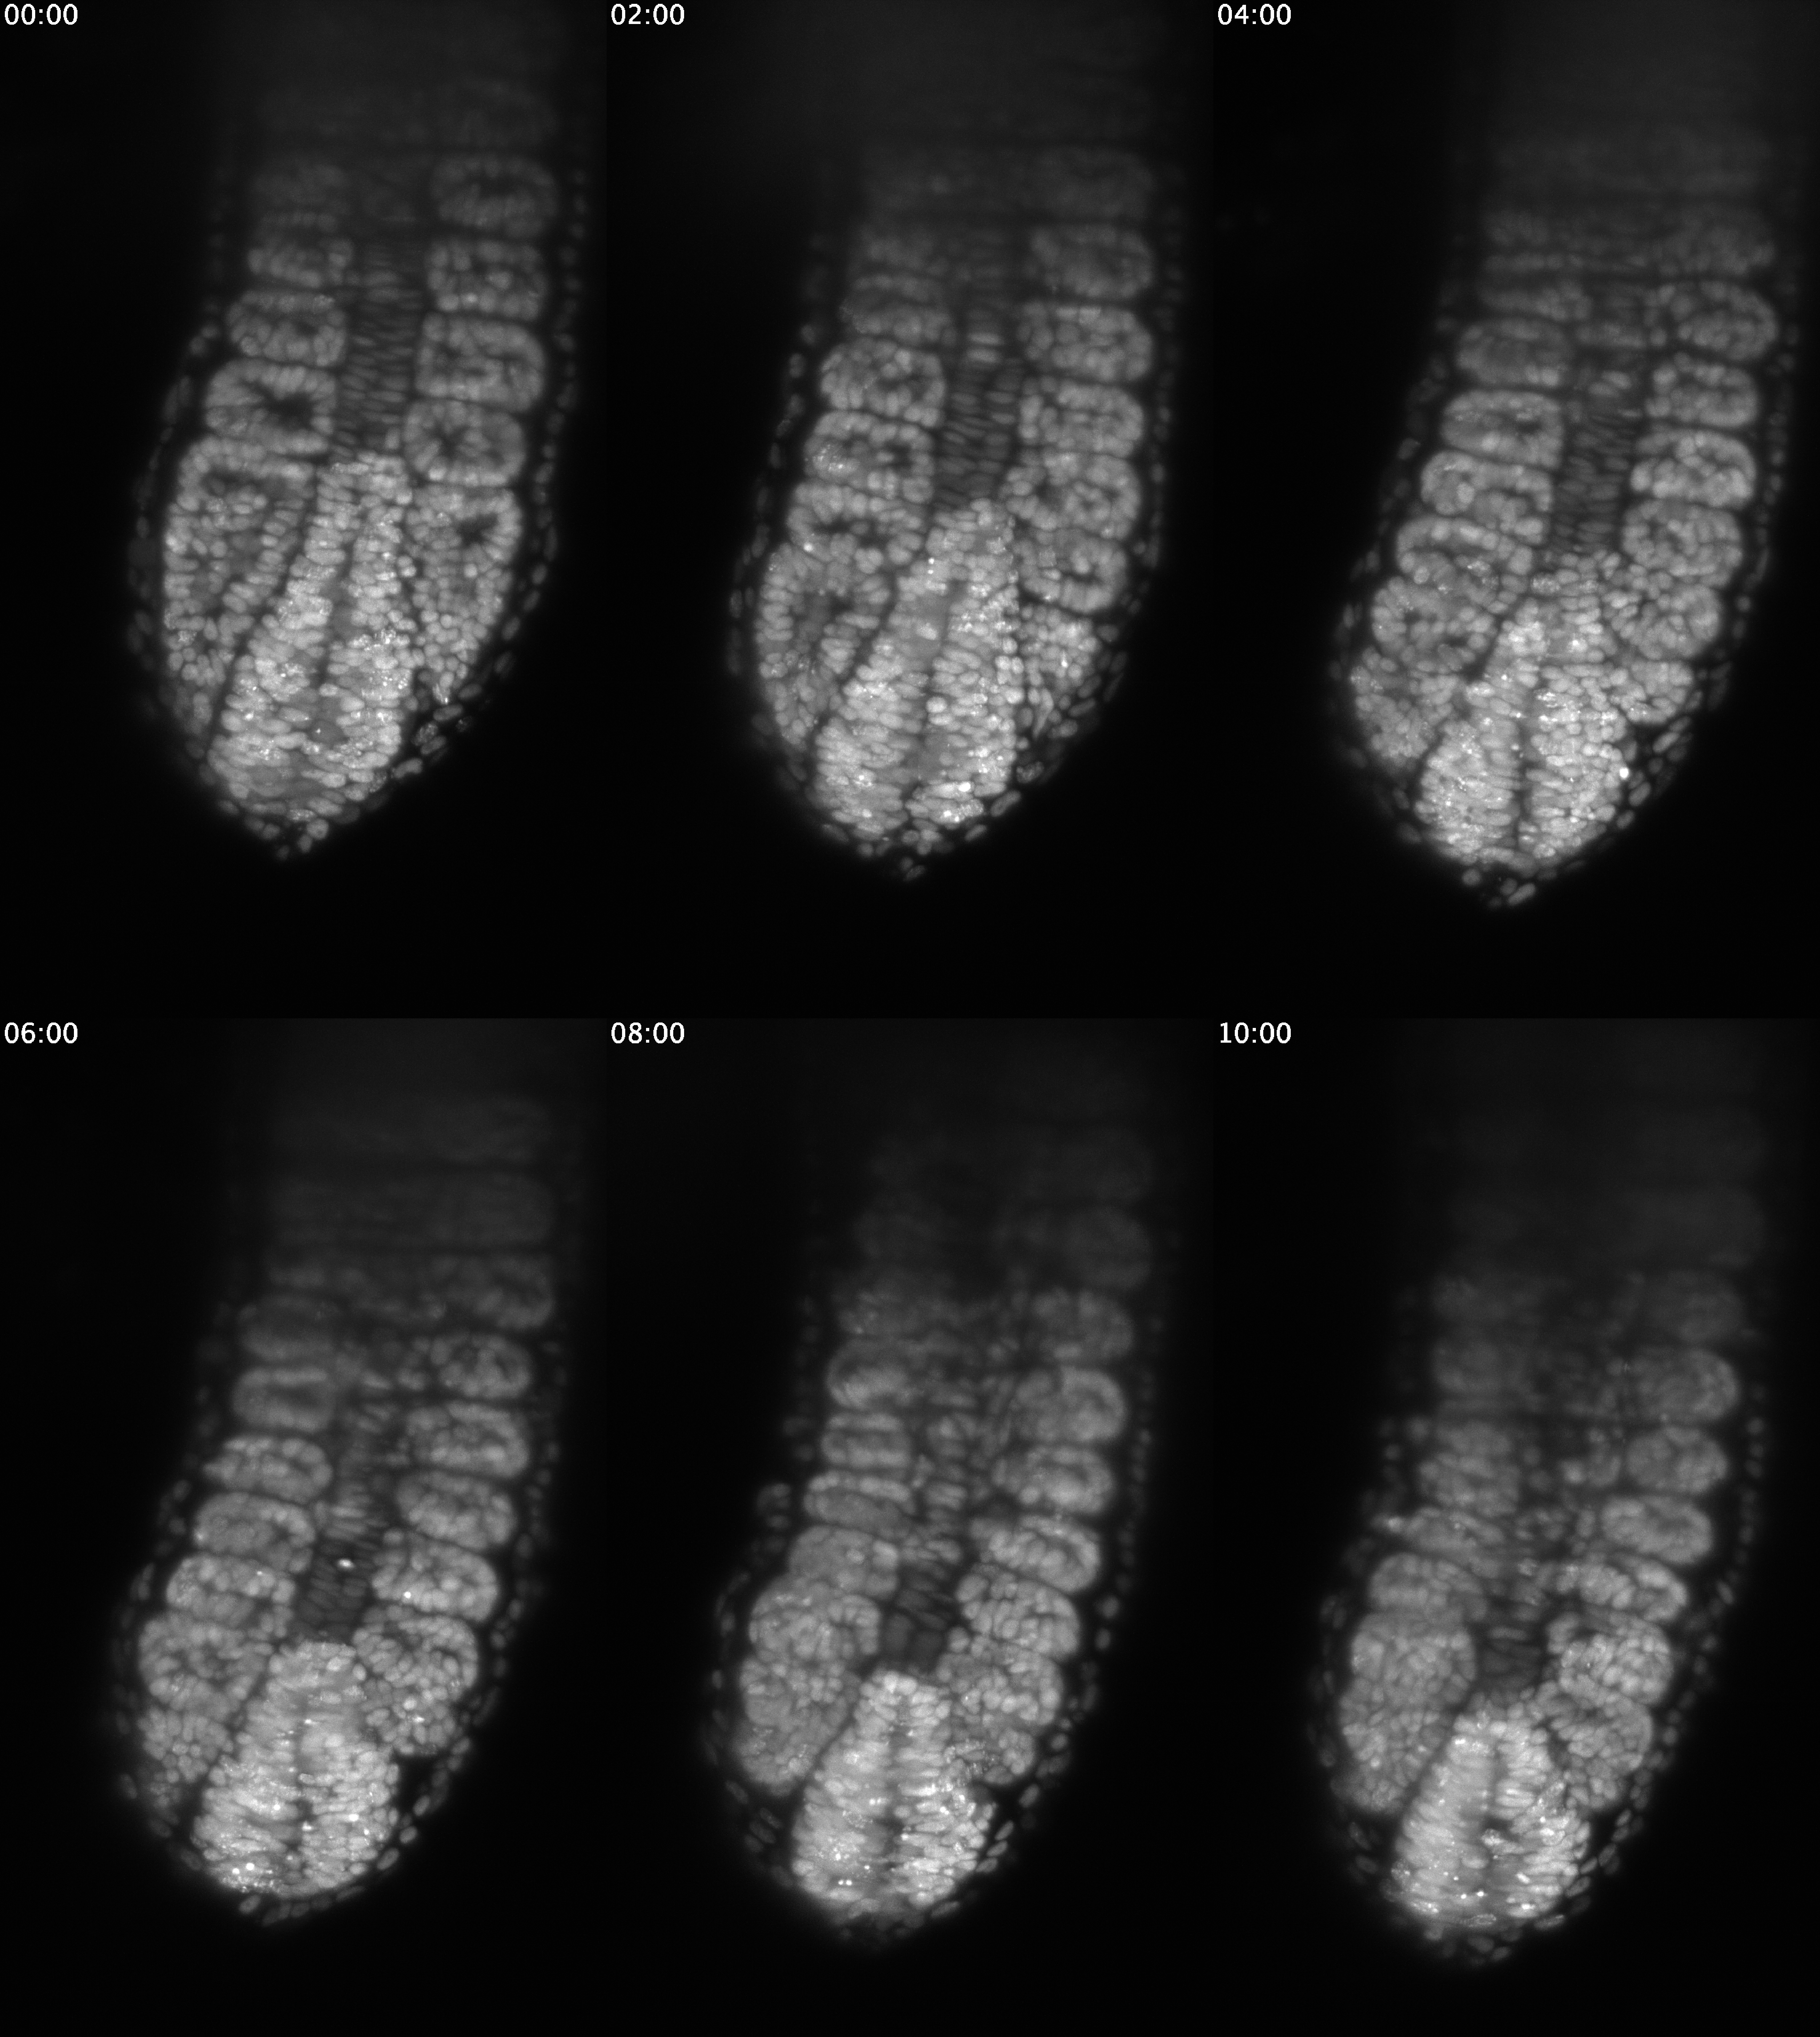
\includegraphics[width=1\linewidth]{figs/somites/ali_fish_seg_compiled} \hfill{}

\caption{Time-stamped images of somite segmentation in medaka, generated by Ali Seleit.}\label{fig:somite-seg-ali}
\end{figure}

The period of somite formation is controlled by a molecular oscillator, known as the `segmentation clock', which drives waves of gene expression in the Notch, fibroblast growth factor (FGF), and Wnt pathways, forming a signalling gradient that regresses towards the tail in concert with axis elongation (Gomez et al. 2008). Over the course of elongation, the wave period increases (i.e.~each somite takes longer to form), and the PSM progressively shrinks until it is exhausted, eventually terminating somite formation (Gomez et al. 2008).

It is not fully understood how the phase waves of the segmentation clock are initially established (Falk et al. 2022). Matsuda et al. (2020) found that period differences between mouse and human occur at the single-cell level (i.e.~not due to intercellular communication), and are driven by biochemical reaction speeds - specifically, mRNA and protein degradation rates, transcription and translation delays, and intron and splicing delays. To identify the genetic basis of these biochemical differences, our collaborators Ali Seleit and Alexander Aulehla at EMBL-Heidelberg used a CRISPR-Case9 knock-in approach (Seleit, Aulehla, and Paix 2021) to establish a medaka \emph{Cab} strain with an endogenous, fluorescing reporter gene (Her7-Venus) for the oscillation signalling pathway. This method allows them to image somite formation and extract quantitative measures for segmentation clock dynamics.

In medaka, it is known that the southern Japanese \emph{Cab} strain and the northern Japanese \emph{Kaga} strain have divergent somite periodicity, where \emph{Kaga}'s tends to be faster, and \emph{Cab}'s slower (\textbf{Figure \ref{fig:F0-Cab-Kaga-HdrR}}).



\begin{figure}
\includegraphics[width=0.5\linewidth]{figs/somites/ali_period_F0_Cab_Kaga} \caption{Comparison of period for three inbred medaka strains (\emph{Cab}, \emph{Kaga} and \emph{HdrR}). Kaga's period is lower, and therefore it takes less time to form each somite than \emph{Cab}. Figure generated by Ali Seleit.}\label{fig:F0-Cab-Kaga-HdrR}
\end{figure}

Our collaborators accordingly set up a one-way F2 cross experiment as described in Chapter \ref{MIKK-F2-cross}, using the reporter-carrying \emph{Cab} strain and the \emph{Kaga} strain as the parental F0 strains, in order to identify genetic loci associated with these differences in clock dynamics. They inter-crossed the hybrid F1 generation to create a sample of 622 F2 individuals, imaged the developing embryos of these F2 samples, and used pyBOAT (Schmal, Mönke, and Granada 2022) to extract the oscillation features during somite development. \textbf{Figure \ref{fig:somite-period-ali}} shows a series of raw images used by pyBOAT to track the elongation of a medaka tail during somitogenesis, with the identified posterior tip of the embryo labelled with a blue circle.



\begin{figure}
\includegraphics[width=0.8\linewidth]{figs/somites/ali_compiled_somite_elong} \caption{Screenshots of vertebral elongation in an F2 individual captured by Ali Seleit during imaging. The blue circle represents the point tracked by pyBOAT over time, generating the quantitative phenotype data on period development used in this study.}\label{fig:somite-period-ali}
\end{figure}

\hypertarget{behaviour}{%
\subsection{Behaviour}\label{behaviour}}

In \textbf{Chapters \ref{Pilot-chap}} and \textbf{\ref{MIKK-F2-chap}} I use medaka as a model organism to explore social genetic effects on bold-type behaviours. Behaviour is a complex trait that is affected by both genes and environment, and for social animals such as humans and medaka, one's social environment is considered likely to constitute a large component of the environmental effect (Ruzzante and Doyle 1990; Young 2008). Apart from social aspects, an organism must face many ``hostile forces of nature'' throughout its life (Buss 1991; Darwin 1859), such as food shortages, predation, harsh climate, and diseases. Adaptive behaviours allow individuals to navigate such dangers and maximise the likelihood of their survival at both the individual and population level (Lima and Dill 1990).

Boldness-shyness is thought to be a fundamental axis of behavioural variation in many species, with an obvious causal relationship to an individual's likelihood of survival, and consequently with natural selection at the population level (Sloan Wilson et al. 1994). It represents an evolutionary trade-off between acquiring benefits (in terms of food or mates) and avoiding harms (in terms of predators or conspecific competitors), with each situation accompanied by its own optimal degree of risk (Lima and Dill 1990). It is both heritable (Svartberg 2002; Culum Brown, Burgess, and Braithwaite 2007), and subject to change following different life experiences or under different environmental conditions (Culum Brown, Burgess, and Braithwaite 2007).

{[}OPEN FIELD AND NOVEL OBJECT IS A GENERIC PARADIGM, NOT JUST FISH. CITE BAUD.{]}

Boldness-shyness has been studied extensively with fish. Shy individuals tend to react to novelty by reducing their activity and becoming more vigilant, whereas bold individuals show higher levels of activity and exploratory behaviour (C. Brown, Jones, and Braithwaite 2007). One assay commonly used to measure this behavioural domain is referred to as the `open field' assay, where fishes are observed while swimming freely in an experimental setting (C. Brown, Jones, and Braithwaite 2007; Laland, Krause, and Brown 2011; Lucon-Xiccato et al. 2022, 2020; Lucon-Xiccato and Bisazza 2017; Matsunaga and Watanabe 2010).

Another is the `novel object' assay, where a novel object is introduced to the fishes' environment to simulate a threat (C. Brown, Jones, and Braithwaite 2007; Schjolden, Stoskhus, and Winberg 2005; Wilson et al. 1993; Dominic Wright, Butlin, and Carlborg 2006; D. Wright et al. 2003). Where both assays were performed on the same fish, the behaviours exhibited were found to be correlated across assays, indicating that both were measuring the same boldness-shyness axis (C. Brown, Jones, and Braithwaite 2007). Both the open field and novel object assay also permit the measurement of habituation, where the response of the fish may change over time after growing accustomed to the new environment or object. Variation in the length of time the fish take to return to a more ``normal'' level of movement may indicate different levels of boldness (Laland, Krause, and Brown 2011).

\hypertarget{social-genetic-effects}{%
\subsubsection{Social genetic effects}\label{social-genetic-effects}}

The experiments described in \textbf{Chapters \ref{Pilot-chap}} and \textbf{\ref{MIKK-F2-chap}} are designed to simulataneously measure both the direct effect of an individual's genes on their behaviour, as we as the indirect effect of their social partner's genes on the focal individual's behaviour, which is also an environmental factor (Baud et al. 2017). Social genetic effects have been shown to exert influence on various traits in mice including anxiety, wound healing, immune function, and body weight (Baud et al. 2017), and various traits related to development and survival in many species of livestock (Ellen et al. 2014). However, in those studies the social interactions were maintained throughout development, and it is unclear whether social genetic effects can still exert influence on adaptive behaviours during discrete, time-limited interactions.

{[}CHECK FLOW{]}

In \textbf{Chapter \ref{MIKK-F2-chap}} I extend the behavioural analysis described in Chapter \ref{Pilot-chap} over the MIKK panel. I then identify the lines that diverged in both (a) their own behaviour; and (b) the level of transmission of their behaviour onto their \emph{\definecolor{iCab_424B4D}{HTML}{424B4D}\textcolor{iCab_424B4D}{iCab}} reference tank partner, and then use them as the parental strains in an F2 cross to attempt to identify the genetic variants associated with those differences.

\hypertarget{poor-transferability-of-polygenic-scores-to-diverse-human-populations}{%
\section{Poor transferability of polygenic scores to diverse human populations}\label{poor-transferability-of-polygenic-scores-to-diverse-human-populations}}

{[}CITE MIKE INOUYE{]}

\textbf{Chapter \ref{Fst-chap}} -- the final chapter of this thesis -- relates to the poor transferability of polygenic scores (\textbf{PRS}) derived from GWAS results when applied to non-European populations. Humans have long sought to use genetic information to predict an individual's likely value for a given trait, in our own species and in other organisms. As already discussed, an individual's phenotypic value at a given point in time is the product of complex interactions between their genome and their environment, beginning from embryonic development and continuing throughout their lifetimes. It is now clear that ``complex'' traits such as height, intelligence, and behaviour are highly polygenic, meaning that they are genetically influenced by hundreds or thousands of genetic variants, each exerting a small effect in one or the other direction along the trait's spectrum (Sella and Barton 2019).

A richer understanding of the cumulative effect of genetic variants on any trait allows for the prediction of the value that an individual is most likely to have for that trait. Of all human traits, diseases are particularly salient; in 2018, the global healthcare industry was valued at US\$8 trillion, and predicted to increase to US\$12 trillion by 2022 ({``The \$11.9 {Trillion Global Healthcare Market}: {Key Opportunities} \& {Strategies} (2014-2022) - {ResearchAndMarkets}.com''} 2019). This strong financial imperative complements the moral imperative to reduce suffering, together driving the question of how to use genetic information to improve human health.

Recent technological developments have made it possible to sequence human genomes at scale, and it is thought that by combining detailed genetic information with with other environmental and phenotypic information (such as lifestyle or clinical factors), clinicians could move towards the practice of ``precision medicine'', where interventions could be tailored to their patients' unique risk profiles (Wray, Goddard, and Visscher 2007). The use of genetic information to predict individuals' values for a trait of interest entails the construction of metrics known as ``polygenic scores'' (\textbf{PGS}). When the trait is a disease, PGS is commonly known as polygenic risk scores (\textbf{PRS}), or genetic risk profiling, but I use the term PGS to encompass both disease and non-disease traits.

\hypertarget{polygenic-scores-pgs-and-gwas}{%
\subsection{Polygenic Scores (PGS) and GWAS}\label{polygenic-scores-pgs-and-gwas}}

\hypertarget{pgs}{%
\subsubsection{PGS}\label{pgs}}

PGS using genetic information alone show modest yet reliable accuracy for the prediction of complex traits (Alicia R. Martin et al. 2019): the correlations between PGS and the trait value as measured by \(R^2\) have reached 0.24 for height (Yengo et al. 2018), and 0.12-0.16 for educational attainment (Okbay et al. 2022). PGS also improve predictions beyond non-genetic clinical models for a variety of health-related traits, including breast cancer (Maas et al. 2016), prostate cancer (Schumacher et al. 2018), and type I diabetes (Sharp et al. 2019). The predictive accuracy of PGS scores can be further improved by combining genetic information with lifestyle and clinical factors, as seen with cardiovascular disease (Khera et al. 2018; Kullo et al. 2016; Natarajan et al. 2017; Paquette et al. 2017; Tikkanen et al. 2013; Sun et al. 2021).

\hypertarget{gwas}{%
\subsubsection{GWAS}\label{gwas}}

Most GWAS have been performed with individuals of European ancestry, despite only constituting around 16\% of the present global population. Although the proportion of participants in GWAS from a non-European background increased from 4\% in 2009 to 16\% in 2016 (Popejoy and Fullerton 2016)), as of 2019, 79\% of all GWAS participants recorded in the GWAS Catalog were of European ancestry, and the proportion of non-European individuals has remained the same or reduced since late 2014 (Alicia R. Martin et al. 2019). This bias extends to PGS studies, where as of 2019, only 67\% of them included only participants of European ancestry, with another 19\% including only East Asian ancestry participants, and only 3.8\% with cohorts of African, Hispanic, or Indigenous ancestry (Duncan et al. 2019).

It is therefore unsurprising that PGS scores are far better at predicting disease risk in individuals of European ancestry than in those of non-European ancestry (Alicia R. Martin et al. 2017; Alicia R. Martin et al. 2019). Indeed, the predictive accuracy of PGS scores decays with genetic divergence of the GWAS ``independent'' or ``test'' sample, from the ``discovery'' or ``training'' sample, as established in both humans (Alicia R. Martin et al. 2017; Alicia R. Martin et al. 2019), and livestock (Clark et al. 2012; Habier et al. 2010; Pszczola et al. 2012).

Compared to PGS scores for those of European ancestry, PGS scores across multiple traits are \textasciitilde64-78\% less accurate for individuals of African ancestry, (Duncan et al. 2019; Alicia R. Martin et al. 2019), \textasciitilde50\% less accurate for individuals of East-Asian ancestry, and \textasciitilde37\% less accurate for individuals of South-Asian ancestry (Alicia R. Martin et al. 2019).

\hypertarget{contributors-to-pgs-non-transferability}{%
\subsection{Contributors to PGS non-transferability}\label{contributors-to-pgs-non-transferability}}

What explains this disparity in predictive value? A number of factors may be responsible, including:

\begin{enumerate}
\def\labelenumi{\arabic{enumi}.}
\item
  The failure of GWAS to identify causal variants that either do not exist or are not identifiable within the ``discovery'' sample, for both technological and methodological reasons (Alicia R. Martin et al. 2019);
\item
  The sample populations may differ in linkage disequilibrium (\textbf{LD}) -- the correlation structure of the genome -- which would change the estimated effect sizes of the causal variants, even when the causal variants themselves are the same (Alicia R. Martin et al. 2019);
\item
  Allele frequencies of the causal variants, and the distribution of the effect sizes of the causal variants, may differ between populations (Alicia R. Martin et al. 2017; Scutari, Mackay, and Balding 2016); and
\item
  The environments and demographies of populations tend to differ. Such differences are often correlated with genetic divergence due to geography, making it difficult to determine whether the associations are driven by the differences between population in their genetics, or their environments (Alicia R. Martin et al. 2019; Kerminen et al. 2019).
\end{enumerate}

The first three factors can degrade predictive performance even in the absence of biological and environmental differences. On the other hand, environmental and demographic differences can drive forces of natural selection can in turn drive differences in causal genetic architecture (Alicia R. Martin et al. 2019).

I will discuss each of these factors in turn before addressing point (3) in this analysis.

\hypertarget{fst-discovery-sec}{%
\subsubsection{Technological and methodological limitations of GWAS}\label{fst-discovery-sec}}

The power to discover a causal variant through GWAS depends on the variant's effect size and frequency in the study population (Alicia R. Martin et al. 2019; Sham et al. 2000). That is to say, the stronger the variant's effect, or the more common it is, the more likely it is to be discovered. Rare variants tend to have stronger effect sizes (Watanabe et al. 2019), likely due to purifying selection (Park et al. 2011), and tend not to be shared across populations (Gravel et al. 2011; 1000. G. P. Consortium et al. 2015). This is particularly relevant for African populations, as they have a much greater level of genetic variance than other populations due to the human species having originated on that continent (1000. G. P. Consortium et al. 2015). Therefore, if GWAS aren't performed on diverse populations, PGS can't take into account the rare variants present in non-European populations that are likely to exert stronger effects on the trait of interest. There are also several other issues that can affect the discoverability of causal variants through GWAS, including the technology used for genotyping, the selection of the cohort, and the necessary exclusion of genotypic outliers.
With respect to genotyping technologies, GWAS often use data from SNP microarrays. These do not sequence the whole genome, but rather a selection (from several hundred thousand to millions) of genetic markers intended to present \emph{common} genetic variation (Porcu et al. 2013), which accordingly tend to neglect rare genetic variants (Uffelmann et al. 2021). To increase the density of genotypes, which would increase the likelihood of refining the association signal and identifying causal variants, researchers often ``impute'' variants that aren't sequenced directly (Porcu et al. 2013). The imputation process involves ``phasing'' the study genotypes onto the genotypes of a ``reference panel'' (McCarthy et al. 2016). However, if the reference panel does not sufficiently represent the population in the study sample, they are likely to miss or incorrectly impute those genotypes (Alicia R. Martin et al. 2019). Again, this is particularly problematic for African populations.

The lack of representation of rare variants in SNP microarrays can be overcome by using next-generation sequencing technologies such as whole-genome sequencing (\textbf{WGS}) and whole-exome sequencing (\textbf{WES}). (The former seeks to sequence the full genome, and the latter of only targets the coding regions of the genome.) These methods are more expensive than SNP microarrays, which hinders their widespread use at scale, and although their costs are continuing to decrease rapidly, there is a question as to whether they return a proportionate benefit in all use cases (Schwarze et al. 2018).

A second limitation is the selection of GWAS cohorts, which can introduce selection and collider biases (Uffelmann et al. 2021). For instance, the UK Biobank, which contains genetic and phenotypic data on 500,000 participants who volunteered for inclusion between 2006 and 2010, tend to be older, female, healthier, and wealthier than non-participants (Fry et al. 2017). This creaties the possibility of confounding genetic associations with environmental factors, which I discuss further in \ref{fst-env-sec} below.

A third limitation is the ``quality control'' step that is required during the GWAS process (Uffelmann et al. 2021). To avoid confounding from population stratification, which can lead to overestimated heritability and biased PGS, GWAS cohorts are filtered to include only those with similar ancestries -- or relative genetic homogeneity -- by clustering individuals through principal component analysis (\textbf{PCA}) of their genotypes, and excluding outliers. I elaborate on the issue of population stratification in section \ref{fst-env-sec} below, but at present, a statistical model for GWAS that can include cohorts with diverse ancestries without the risk of serious confounding is yet to be developed (Berg et al. 2019).

\hypertarget{differences-in-ld}{%
\subsubsection{Differences in LD}\label{differences-in-ld}}

Because GWAS SNP markers are often not the causal variants themselves, but merely in physical proximity to them, the estimated effect size of a SNP marker depends on the extent to which it is in LD with the causal variant (Mostafavi et al. 2020; Pritchard and Przeworski 2001). To illustrate the problem, if a SNP has an LD \(r^2\) with a causal variant of 0.8 in the discovery population and 0.6 in the target population, it would explain 25\% = (1 - 0.6/0.8) less trait variation in the target population, and would therefore be less predictive (Ying Wang et al. 2020).

These differences in effect-size estimates may typically be small for most regions of the genome, but as PGS sum across all such effects, they aggregate these population differences (Alicia R. Martin et al. 2019; Berg et al. 2019). Previous empirical and simulation studies have shown that accuracy of PGS scores decay with increased genetic differentiation (\(F_{ST}\) -- described below in \ref{Fst-descr}) and LD differences between populations (Habier et al. 2010; Pszczola et al. 2012; Scutari, Mackay, and Balding 2016; Ying Wang et al. 2020). The issue may be addressed to a degree by using LD information from an external reference panel as a prior to infer the posterior mean effect size of a genetic variant -- Vilhjálmsson et al. (2015) demonstrated through simulations that this could improve PGS predictive accuracy. Yet the most appropriate means of deal with differences between populations in LD remains an active area of research (Duncan et al. 2019).

\hypertarget{differences-in-allele-frequencies}{%
\subsubsection{Differences in allele frequencies}\label{differences-in-allele-frequencies}}

Causal variants can differ in both frequency and effect size between different ancestry groups, e.g.~for lactase persistence (S'egurel and Bon 2017), or skin pigmentation (Adhikari et al. 2019). If a causal allele is rare in the GWAS discovery population, even if it is discovered (see \ref{fst-discovery-sec}), it is likely to have noisy effect size estimates, and therefore likely to inaccurately estimate its effect size in a different population where it exists at a higher frequency.

Differences in allele frequencies between populations can arise through random genetic drift, or be driven by selective pressures towards the trait optima for a given environment (Harpak and Przeworski 2021). However, evolutionary biologists have found that differences between populations in the mean values for traits tend to occur through small, coordinated shifts in their allele frequencies (Berg et al. 2019; Edge and Coop 2019). In Chapter \ref{Fst-chap}, I explore the differences in allele frequencies across populations for all polygenic traits in the GWAS Catalog, and confirm that with few exceptions -- including skin pigmentation, and HIV viral load -- the differences in allele frequencies between populations tends to be small.

\hypertarget{fst-env-sec}{%
\subsubsection{Differences in environment}\label{fst-env-sec}}

Genes continuously interact with each other (GxG, or ``epistasis'' (Gros, Le Nagard, and Tenaillon 2009)), the genes of one's parents (``genetic nurture'', Kong et al. (2018)) or social companions (``social genetic effects'') (Domingue et al. 2018; Baud et al. 2017),\footnote{As also explored in Chapters \ref{Pilot-chap} and \ref{MIKK-F2-chap}} and the wider non-genetic environment (GxE).

The respective contributions of genetics and environment to traits with social value -- such as intelligence -- is highly contentious, especially when there are apparent differences between populations in the mean values for those traits. PGS measure the proportion of variance within a population that is explained by genetics. Because PRS summarises a \emph{proportion} of the total variance, when studying a population that is subject to greater environmental variation, the variance attributable to genetic factors will proportionately reduce. The corollary being that when studying a population where the environment is held constant, the proportion of variance for that trait that is explained by genetic factors will approach 1. Therefore, increases in the amount of environmental variance that a population is exposed to will reduce the accuracy of PGS predictions when applied to that population.

Different environments are also often correlated with population structure (Berg et al. 2019). For example, in East Asia, there is a greater proportion of individuals of East-Asian ancestry than there is of European ancestry, and \emph{vice versa} in Europe. Those East-Asian individuals will therefore tend to share more of their genetic background with each other than with Europeans, and that population structure will be correlated with the different environments that exist in East Asia compared to Europe. This makes it difficult to determine whether it is the differences in their environments or the differences in their genetics that is driving the discrepancies between the mean values for traits between those populations. These complexities are unlikely to be resolved in the near future, which makes it attractive to turn to model organisms to address more basic biological questions regarding GxE in relation to complex traits (Andersson and Georges 2004), as we have done with respect to behaviour in Chapters \ref{Pilot-chap} and \ref{MIKK-F2-chap}.

\hypertarget{Fst-descr}{%
\subsection{\texorpdfstring{\(F_{ST}\)}{F\_\{ST\}}}\label{Fst-descr}}

The widely-used fixation index (\(F_{ST}\)) was introduced independently by Sewall Wright (S. Wright 1949) and Gustave Malécot (Mal'ecot 1948) as a metric for measuring the genetic diversity between populations.\footnote{In Wright's notation, \(F\) refers to ``fixation'' of an allele, and \(_{ST}\) refers to ``subpopulations within the total population''.} It quantifies the relative variance in allele frequency between groups compared to within groups, reflecting the combined effects of genetic drift, migration, mutation, and selection (Holsinger and Weir 2009). The metric ranges from 0 to 1, where loci with high \(F_{ST}\) values -- that is, loci with a large relative between-group variance in allele frequencies -- may have been subject to selection or different demographic processes (Holsinger and Weir 2009). The metric has customarily been used to identify regions of the genome have been subject to diversifying selection (Akey et al. 2002; Guo, Dey, and Holsinger 2009; Weir et al. 2005).

\hypertarget{refs}{}
\begin{CSLReferences}{1}{0}
\leavevmode\vadjust pre{\hypertarget{ref-adhikariGWASLatinAmericans2019}{}}%
Adhikari, Kaustubh, Javier Mendoza-Revilla, Anood Sohail, Macarena Fuentes-Guajardo, Jodie Lampert, Juan Camilo Chac'on-Duque, Malena Hurtado, et al. 2019. {``A {GWAS} in {Latin Americans} Highlights the Convergent Evolution of Lighter Skin Pigmentation in {Eurasia}.''} \emph{Nature Communications} 10 (1, 1): 358. \url{https://doi.org/10.1038/s41467-018-08147-0}.

\leavevmode\vadjust pre{\hypertarget{ref-aidaInheritanceColorFreshWater1921}{}}%
Aida, Tatuo. 1921. {``On the {Inheritance} of {Color} in a {Fresh-Water Fish}, {Aplocheilus Latipes Temmick} and {Schlegel}, with {Special Reference} to {Sex-Linked Inheritance}.''} \emph{Genetics} 6 (6): 554--73. \url{https://www.ncbi.nlm.nih.gov/pmc/articles/PMC1200522/}.

\leavevmode\vadjust pre{\hypertarget{ref-airdBloodGroupsRelation1954}{}}%
Aird, Ian, H. H. Bentall, J. A. Mehigan, and J. A. Fraser Roberts. 1954. {``The {Blood Groups} in {Relation} to {Peptic Ulceration} and {Carcinoma} of {Colon}, {Rectum}, {Breast}, and {Bronchus}.''} \emph{Br Med J} 2 (4883): 315--21. \url{https://doi.org/10.1136/bmj.2.4883.315}.

\leavevmode\vadjust pre{\hypertarget{ref-akeyInterrogatingHighDensitySNP2002}{}}%
Akey, Joshua M., Ge Zhang, Kun Zhang, Li Jin, and Mark D. Shriver. 2002. {``Interrogating a {High-Density SNP Map} for {Signatures} of {Natural Selection}.''} \emph{Genome Research} 12 (12): 1805--14. \url{https://doi.org/10.1101/gr.631202}.

\leavevmode\vadjust pre{\hypertarget{ref-altshulerGeneticMappingHuman2008}{}}%
Altshuler, David, Mark J. Daly, and Eric S. Lander. 2008. {``Genetic {Mapping} in {Human Disease}.''} \emph{Science} 322 (5903): 881--88. \url{https://doi.org/10.1126/science.1156409}.

\leavevmode\vadjust pre{\hypertarget{ref-anderssonDomesticanimalGenomicsDeciphering2004}{}}%
Andersson, Leif, and Michel Georges. 2004. {``Domestic-Animal Genomics: Deciphering the Genetics of Complex Traits.''} \emph{Nature Reviews Genetics} 5 (3, 3): 202--12. \url{https://doi.org/10.1038/nrg1294}.

\leavevmode\vadjust pre{\hypertarget{ref-aristotleGenerationAnimals2021}{}}%
Aristotle. 2021. \emph{On the {Generation} of {Animals}}. {Good Press}. \url{https://books.google.com?id=aLUqEAAAQBAJ}.

\leavevmode\vadjust pre{\hypertarget{ref-armstrongEnglishParsonnaturalistCompanionship2000}{}}%
Armstrong, Patrick. 2000. \emph{The {English Parson-naturalist}: {A Companionship Between Science} and {Religion}}. {Gracewing Publishing}. \url{https://books.google.com?id=hB0hEc4CN3wC}.

\leavevmode\vadjust pre{\hypertarget{ref-badiouPlatoRepublic2013}{}}%
Badiou, Alain. 2013. \emph{Plato's {Republic}}. {John Wiley \& Sons}.

\leavevmode\vadjust pre{\hypertarget{ref-bancroftPartIntroductionGouldian}{}}%
Bancroft, Paul. n.d. {``Part 1: {An} Introduction to the {Gouldian} Finch - {Planet Aviary}.''} Accessed August 22, 2022. \url{https://planetaviary.com/part-1-an-introduction-to-the-gouldian-finch/}.

\leavevmode\vadjust pre{\hypertarget{ref-bartonSewallWrightEvolution2016}{}}%
Barton, Nicholas H. 2016. {``Sewall {Wright} on {Evolution} in {Mendelian Populations} and the {`{Shifting Balance}'}.''} \emph{Genetics} 202 (1): 3--4. \url{https://doi.org/10.1534/genetics.115.184796}.

\leavevmode\vadjust pre{\hypertarget{ref-batesonMaterialsStudyVariation1894}{}}%
Bateson, William. 1894. \emph{Materials for the {Study} of {Variation}: {Treated} with {Especial Regard} to {Discontinuity} in the {Origin} of {Species}}. {Macmillan and Company}. \url{https://books.google.com?id=_HIZAAAAYAAJ}.

\leavevmode\vadjust pre{\hypertarget{ref-batesonMendelPrinciplesHeredity1909}{}}%
---------. 1909. {``Mendel's {Principles} of {Heredity}: {Cambridge University Press}.''} \emph{März 1909; 2nd Impr} 3: 1913.

\leavevmode\vadjust pre{\hypertarget{ref-baudGeneticVariationSocial2017}{}}%
Baud, Amelie, Megan K. Mulligan, Francesco Paolo Casale, Jesse F. Ingels, Casey J. Bohl, Jacques Callebert, Jean-Marie Launay, et al. 2017. {``Genetic {Variation} in the {Social Environment Contributes} to {Health} and {Disease}.''} \emph{PLOS Genetics} 13 (1): e1006498. \url{https://doi.org/10.1371/journal.pgen.1006498}.

\leavevmode\vadjust pre{\hypertarget{ref-bergReducedSignalPolygenic2019}{}}%
Berg, Jeremy J, Arbel Harpak, Nasa Sinnott-Armstrong, Anja Moltke Joergensen, Hakhamanesh Mostafavi, Yair Field, Evan August Boyle, et al. 2019. {``Reduced Signal for Polygenic Adaptation of Height in {UK Biobank}.''} Edited by Magnus Nordborg, Mark I McCarthy, Magnus Nordborg, Nicholas H Barton, and Joachim Hermisson. \emph{eLife} 8 (March): e39725. \url{https://doi.org/10.7554/eLife.39725}.

\leavevmode\vadjust pre{\hypertarget{ref-bergelsonIdentifyingGenesUnderlying2010}{}}%
Bergelson, Joy, and Fabrice Roux. 2010. {``Towards Identifying Genes Underlying Ecologically Relevant Traits in {Arabidopsis} Thaliana.''} \emph{Nature Reviews Genetics} 11 (12, 12): 867--79. \url{https://doi.org/10.1038/nrg2896}.

\leavevmode\vadjust pre{\hypertarget{ref-brownCorrelationBoldnessBody2007}{}}%
Brown, C., F. Jones, and V. A. Braithwaite. 2007. {``Correlation Between Boldness and Body Mass in Natural Populations of the Poeciliid {Brachyrhaphis} Episcopi.''} \emph{Journal of Fish Biology} 71 (6): 1590--1601. \url{https://doi.org/10.1111/j.1095-8649.2007.01627.x}.

\leavevmode\vadjust pre{\hypertarget{ref-brownHeritableExperientialEffects2007}{}}%
Brown, Culum, Fiona Burgess, and Victoria A. Braithwaite. 2007. {``Heritable and Experiential Effects on Boldness in a Tropical Poeciliid.''} \emph{Behavioral Ecology and Sociobiology} 62 (2): 237--43. \url{https://doi.org/10.1007/s00265-007-0458-3}.

\leavevmode\vadjust pre{\hypertarget{ref-bussEvolutionaryPersonalityPsychology1991}{}}%
Buss, David M. 1991. {``Evolutionary Personality Psychology.''} \emph{Annual Review of Psychology} 42: 459--91. \url{https://doi.org/10.1146/annurev.ps.42.020191.002331}.

\leavevmode\vadjust pre{\hypertarget{ref-caballeroQuantitativeGenetics2020}{}}%
Caballero, Armando. 2020. \emph{Quantitative {Genetics}}. {Cambridge University Press}. \url{https://books.google.com?id=yOfWDwAAQBAJ}.

\leavevmode\vadjust pre{\hypertarget{ref-campbellKingJamesBible2010}{}}%
Campbell, Gordon. 2010. \emph{King {James Bible}: 400th {Anniversary Edition}}. {OUP Oxford}.

\leavevmode\vadjust pre{\hypertarget{ref-clarkImportanceInformationRelatives2012}{}}%
Clark, Samuel A., John M. Hickey, Hans D. Daetwyler, and Julius HJ van der Werf. 2012. {``The Importance of Information on Relatives for the Prediction of Genomic Breeding Values and the Implications for the Makeup of Reference Data Sets in Livestock Breeding Schemes.''} \emph{Genetics Selection Evolution} 44 (1): 4. \url{https://doi.org/10.1186/1297-9686-44-4}.

\leavevmode\vadjust pre{\hypertarget{ref-collinsVariationsThemeCataloging1997}{}}%
Collins, Francis S., Mark S. Guyer, and Aravinda Chakravarti. 1997. {``Variations on a {Theme}: {Cataloging Human DNA Sequence Variation}.''} \emph{Science} 278 (5343): 1580--81. \url{https://doi.org/10.1126/science.278.5343.1580}.

\leavevmode\vadjust pre{\hypertarget{ref-batesonPhoto}{}}%
Commons, Wikimedia. 2017a. {``File:Bateson2.jpg --- Wikimedia Commons{,} the Free Media Repository.''} \url{/url\%7Bhttps://commons.wikimedia.org/w/index.php?title=File:Bateson2.jpg\&oldid=255958176\%7D}.

\leavevmode\vadjust pre{\hypertarget{ref-charlesDarwinYoung}{}}%
---------. 2017b. {``File:charles Darwin by g. Richmond.png --- Wikimedia Commons{,} the Free Media Repository.''} \url{/url\%7Bhttps://commons.wikimedia.org/w/index.php?title=File:Charles_Darwin_by_G._Richmond.png\&oldid=260695102\%7D}.

\leavevmode\vadjust pre{\hypertarget{ref-homunculusImage}{}}%
---------. 2019. {``File:preformation.GIF --- Wikimedia Commons{,} the Free Media Repository.''} \url{/url\%7Bhttps://commons.wikimedia.org/w/index.php?title=File:Preformation.GIF\&oldid=372547016\%7D}.

\leavevmode\vadjust pre{\hypertarget{ref-pearsonPhoto}{}}%
---------. 2020. {``File:karl Pearson, 1910.jpg --- Wikimedia Commons{,} the Free Media Repository.''} \url{/url\%7Bhttps://commons.wikimedia.org/w/index.php?title=File:Karl_Pearson,_1910.jpg\&oldid=477532248\%7D}.

\leavevmode\vadjust pre{\hypertarget{ref-galtonPhoto}{}}%
---------. 2021a. {``File:francis Galton 1850s.jpg --- Wikimedia Commons{,} the Free Media Repository.''} \url{/url\%7Bhttps://commons.wikimedia.org/w/index.php?title=File:Francis_Galton_1850s.jpg\&oldid=569302173\%7D}.

\leavevmode\vadjust pre{\hypertarget{ref-mendelPhoto}{}}%
---------. 2021b. {``File:gregor Mendel 2.jpg --- Wikimedia Commons{,} the Free Media Repository.''} \url{/url\%7Bhttps://commons.wikimedia.org/w/index.php?title=File:Gregor_Mendel_2.jpg\&oldid=534728192\%7D}.

\leavevmode\vadjust pre{\hypertarget{ref-fisherPhoto}{}}%
---------. 2021c. {``File:Youngronaldfisher2.JPG --- Wikimedia Commons{,} the Free Media Repository.''} \url{/url\%7Bhttps://commons.wikimedia.org/w/index.php?title=File:Youngronaldfisher2.JPG\&oldid=614548490\%7D}.

\leavevmode\vadjust pre{\hypertarget{ref-alfredWallace1895}{}}%
---------. 2022a. {``File:alfred-Russel-Wallace-C1895.jpg --- Wikimedia Commons{,} the Free Media Repository.''} \url{https://commons.wikimedia.org/w/index.php?title=File:Alfred-Russel-Wallace-c1895.jpg\&oldid=642853479}.

\leavevmode\vadjust pre{\hypertarget{ref-darwinFinches}{}}%
---------. 2022b. {``File:darwin's Finches by Gould.jpg --- Wikimedia Commons{,} the Free Media Repository.''} \url{/url\%7Bhttps://commons.wikimedia.org/w/index.php?title=File:Darwin\%27s_finches_by_Gould.jpg\&oldid=643906085\%7D}.

\leavevmode\vadjust pre{\hypertarget{ref-lamarck1802}{}}%
---------. 2022c. {``File:jean-Baptiste de Lamarck.jpg --- Wikimedia Commons{,} the Free Media Repository.''} \url{/url\%7Bhttps://commons.wikimedia.org/w/index.php?title=File:Jean-Baptiste_de_Lamarck.jpg\&oldid=641428959\%7D}.

\leavevmode\vadjust pre{\hypertarget{ref-10002015global}{}}%
Consortium, 1000 Genomes Project et al. 2015. {``A Global Reference for Human Genetic Variation.''} \emph{Nature} 526 (7571): 68.

\leavevmode\vadjust pre{\hypertarget{ref-internationalhumangenomesequencingconsortiumInitialSequencingAnalysis2001a}{}}%
Consortium, International Human Genome Sequencing. 2001. {``Initial Sequencing and Analysis of the Human Genome.''} \emph{Nature} 409 (6822, 6822): 860--921. \url{https://doi.org/10.1038/35057062}.

\leavevmode\vadjust pre{\hypertarget{ref-coyneTheodosiusDobzhanskyHybrid2016}{}}%
Coyne, Jerry A. 2016. {``Theodosius {Dobzhansky} on {Hybrid Sterility} and {Speciation}.''} \emph{Genetics} 202 (1): 5--7. \url{https://doi.org/10.1534/genetics.115.184770}.

\leavevmode\vadjust pre{\hypertarget{ref-darwinOriginSpeciesMeans1859}{}}%
Darwin, Charles. 1859. \emph{On the {Origin} of {Species} by {Means} of {Natural Selection}, {Or}, {The Preservation} of {Favoured Races} in the {Struggle} for {Life}}. {J. Murray}. \url{https://books.google.com?id=gGUYt2PsDJcC}.

\leavevmode\vadjust pre{\hypertarget{ref-darwinNaturalistVoyageJournal1882}{}}%
---------. 1882. \emph{A {Naturalist}'s {Voyage}: {Journal} of {Researches Into} the {Natural History} and {Geology} of the {Countries Visited During} the {Voyage} of {H}.{M}.{S}. {Beagle} : With {Maps} and {Illustrations}}. {Murray}. \url{https://books.google.com?id=JyR7HY3FMtkC}.

\leavevmode\vadjust pre{\hypertarget{ref-darwinCharlesDarwinLetters1998}{}}%
---------. 1998. \emph{Charles {Darwin}'s {Letters}: {A Selection}, 1825-1859}. {Cambridge University Press}. \url{https://books.google.com?id=E2TTcP6KUHgC}.

\leavevmode\vadjust pre{\hypertarget{ref-darwinAutobiographyCharlesDarwin2019}{}}%
---------. 2019. \emph{The {Autobiography} of {Charles Darwin}}. {BoD -- Books on Demand}. \url{https://books.google.com?id=t_SxDwAAQBAJ}.

\leavevmode\vadjust pre{\hypertarget{ref-DNAThenNow}{}}%
{``{DNA} Then and Now.''} n.d. Accessed August 30, 2022. \url{https://undsci.berkeley.edu/article/0_0_0/dna_14}.

\leavevmode\vadjust pre{\hypertarget{ref-domingueSocialGenomeFriends2018}{}}%
Domingue, Benjamin W., Daniel W. Belsky, Jason M. Fletcher, Dalton Conley, Jason D. Boardman, and Kathleen Mullan Harris. 2018. {``The Social Genome of Friends and Schoolmates in the {National Longitudinal Study} of {Adolescent} to {Adult Health}.''} \emph{Proceedings of the National Academy of Sciences} 115 (4): 702--7. \url{https://doi.org/10.1073/pnas.1711803115}.

\leavevmode\vadjust pre{\hypertarget{ref-drueryExperimentsPlantHybridization1901}{}}%
Druery, C. T., and William Bateson. 1901. {``Experiments in Plant Hybridization.''} \emph{Journal of the Royal Horticultural Society} 26: 1--32.

\leavevmode\vadjust pre{\hypertarget{ref-duncanAnalysisPolygenicRisk2019}{}}%
Duncan, L., H. Shen, B. Gelaye, J. Meijsen, K. Ressler, M. Feldman, R. Peterson, and B. Domingue. 2019. {``Analysis of Polygenic Risk Score Usage and Performance in Diverse Human Populations.''} \emph{Nature Communications} 10 (1, 1): 3328. \url{https://doi.org/10.1038/s41467-019-11112-0}.

\leavevmode\vadjust pre{\hypertarget{ref-eatonQuartercenturyInbreedingGuineapigs1932}{}}%
Eaton, Orson N. 1932. {``A Quarter-Century of Inbreeding in Guinea-Pigs.''} \emph{Journal of Experimental Zoology} 63 (2): 261--90. \url{https://doi.org/10.1002/jez.1400630202}.

\leavevmode\vadjust pre{\hypertarget{ref-edgeReconstructingHistoryPolygenic2019}{}}%
Edge, Michael D, and Graham Coop. 2019. {``Reconstructing the {History} of {Polygenic Scores Using Coalescent Trees}.''} \emph{Genetics} 211 (1): 235--62. \url{https://doi.org/10.1534/genetics.118.301687}.

\leavevmode\vadjust pre{\hypertarget{ref-ellenProspectsSelectionSocial2014}{}}%
Ellen, Esther D., T. Bas Rodenburg, Gerard A. A. Albers, J. Elizabeth Bolhuis, Irene Camerlink, Naomi Duijvesteijn, Egbert F. Knol, et al. 2014. {``The Prospects of Selection for Social Genetic Effects to Improve Welfare and Productivity in Livestock.''} \emph{Frontiers in Genetics} 5. \url{https://www.frontiersin.org/articles/10.3389/fgene.2014.00377}.

\leavevmode\vadjust pre{\hypertarget{ref-evansQTLGeneElegans2021}{}}%
Evans, Kathryn S., Marijke H. van Wijk, Patrick T. McGrath, Erik C. Andersen, and Mark G. Sterken. 2021. {``From {QTL} to Gene: {C}. Elegans Facilitates Discoveries of the Genetic Mechanisms Underlying Natural Variation.''} \emph{Trends in Genetics} 37 (10): 933--47. \url{https://doi.org/10.1016/j.tig.2021.06.005}.

\leavevmode\vadjust pre{\hypertarget{ref-ewensTransmissionDisequilibriumTest1995}{}}%
Ewens, W J, and R S Spielman. 1995. {``The Transmission/Disequilibrium Test: History, Subdivision, and Admixture.''} \emph{American Journal of Human Genetics} 57 (2): 455--64. \url{https://www.ncbi.nlm.nih.gov/pmc/articles/PMC1801556/}.

\leavevmode\vadjust pre{\hypertarget{ref-falconerIntroductionQuantitativeGenetics1996}{}}%
Falconer, D. S., and T. F. C. Mackay. 1996. \emph{Introduction to Quantitative Genetics}. {UK: Longman Group}.

\leavevmode\vadjust pre{\hypertarget{ref-falkImagingOnsetOscillatory2022}{}}%
Falk, Henning J, Takehito Tomita, Gregor Mönke, Katie McDole, and Alexander Aulehla. 2022. {``Imaging the Onset of Oscillatory Signaling Dynamics During Mouse Embryo Gastrulation.''} \emph{Development (Cambridge, England)} 149 (13): dev200083. \url{https://doi.org/10.1242/dev.200083}.

\leavevmode\vadjust pre{\hypertarget{ref-fisherXVCorrelationRelatives1919}{}}%
Fisher, R. A. 1919. {``{XV}.---{The Correlation} Between {Relatives} on the {Supposition} of {Mendelian Inheritance}.''} January. \url{https://doi.org/10.1017/s0080456800012163}.

\leavevmode\vadjust pre{\hypertarget{ref-fisherStudiesCropVariation1923}{}}%
Fisher, R. A., and W. A. Mackenzie. 1923. {``Studies in Crop Variation. {II}. {The} Manurial Response of Different Potato Varieties.''} \emph{The Journal of Agricultural Science} 13 (3): 311--20. \url{https://doi.org/10.1017/S0021859600003592}.

\leavevmode\vadjust pre{\hypertarget{ref-fisherProbableErrorCoefficient1921}{}}%
Fisher, Ronald Aylmer. 1921. {``On the{"} {Probable Error}{"} of a {Coefficient} of {Correlation Deduced} from a {Small Sample}.''}

\leavevmode\vadjust pre{\hypertarget{ref-fisherStatisticalMethodsResearch1925}{}}%
---------. 1925. \emph{Statistical {Methods} for {Research Workers}}. {Oliver and Boyd}. \url{https://books.google.com?id=1NApzwEACAAJ}.

\leavevmode\vadjust pre{\hypertarget{ref-fitzgeraldMedakaInbredKiyosuKarlsruhe2022}{}}%
Fitzgerald, Tomas, Ian Brettell, Adrien Leger, Nadeshda Wolf, Natalja Kusminski, Jack Monahan, Carl Barton, et al. 2022. {``The {Medaka Inbred Kiyosu-Karlsruhe} ({MIKK}) Panel.''} \emph{Genome Biology} 23 (1): 59. \url{https://doi.org/10.1186/s13059-022-02623-z}.

\leavevmode\vadjust pre{\hypertarget{ref-franklinMolecularConfigurationSodium1953}{}}%
Franklin, Rosalind E., and Raymond G. Gosling. 1953. {``Molecular Configuration in Sodium Thymonucleate.''} \emph{Nature} 171 (4356): 740--41.

\leavevmode\vadjust pre{\hypertarget{ref-fryComparisonSociodemographicHealthRelated2017}{}}%
Fry, Anna, Thomas J Littlejohns, Cathie Sudlow, Nicola Doherty, Ligia Adamska, Tim Sprosen, Rory Collins, and Naomi E Allen. 2017. {``Comparison of {Sociodemographic} and {Health-Related Characteristics} of {UK Biobank Participants With Those} of the {General Population}.''} \emph{American Journal of Epidemiology} 186 (9): 1026--34. \url{https://doi.org/10.1093/aje/kwx246}.

\leavevmode\vadjust pre{\hypertarget{ref-fukamachi100YearsMedaka2021}{}}%
Fukamachi, Shoji, and Kiyoshi Naruse. 2021. {``100 Years Since the Medaka's International Debut: {Aida}'s Legacy.''} {Genes to Genomes}. August 20, 2021. \url{https://genestogenomes.org/100-years-since-the-medakas-international-debut-aidas-legacy/}.

\leavevmode\vadjust pre{\hypertarget{ref-galtonMenScienceTheir1874a}{}}%
Galton, Francis. 1874. {``On {Men} of {Science}, Their {Nature} and Their {Nurture}.''} In \emph{Proceedings of the {Royal Institution} of {Great Britain}}, 7:227--36.

\leavevmode\vadjust pre{\hypertarget{ref-galtonEugenicsItsDefinition1904}{}}%
---------. 1904. {``Eugenics: {Its Definition}, {Scope}, and {Aims}.''} \emph{American Journal of Sociology} 10 (1): 1--25. \url{https://doi.org/10.1086/211280}.

\leavevmode\vadjust pre{\hypertarget{ref-gomezControlSegmentNumber2008}{}}%
Gomez, C'eline, Ertuğrul M. Özbudak, Joshua Wunderlich, Diana Baumann, Julian Lewis, and Olivier Pourqui'e. 2008. {``Control of Segment Number in Vertebrate Embryos.''} \emph{Nature} 454 (7202, 7202): 335--39. \url{https://doi.org/10.1038/nature07020}.

\leavevmode\vadjust pre{\hypertarget{ref-goodnightSewallWrightSeven2014}{}}%
Goodnight, Charles. 2014. {``Sewall {Wright}'s {Seven Generalizations} about {Populations}.''} {Evolution in Structured Populations}. May 22, 2014. \url{https://blog.uvm.edu/cgoodnig/2014/05/22/sewall-wrights-seven-generalizations-about-populations/}.

\leavevmode\vadjust pre{\hypertarget{ref-gravel2011demographic}{}}%
Gravel, Simon, Brenna M Henn, Ryan N Gutenkunst, Amit R Indap, Gabor T Marth, Andrew G Clark, Fuli Yu, et al. 2011. {``Demographic History and Rare Allele Sharing Among Human Populations.''} \emph{Proceedings of the National Academy of Sciences} 108 (29): 11983--88. \url{https://doi.org/10.1073/pnas.1019276108}.

\leavevmode\vadjust pre{\hypertarget{ref-gridleyLongShortIt2006}{}}%
Gridley, Thomas. 2006. {``The Long and Short of It: {Somite} Formation in Mice.''} \emph{Developmental Dynamics} 235 (9): 2330--36. \url{https://doi.org/10.1002/dvdy.20850}.

\leavevmode\vadjust pre{\hypertarget{ref-grosEvolutionEpistasisIts2009}{}}%
Gros, Pierre-Alexis, Herv'e Le Nagard, and Olivier Tenaillon. 2009. {``The {Evolution} of {Epistasis} and {Its Links With Genetic Robustness}, {Complexity} and {Drift} in a {Phenotypic Model} of {Adaptation}.''} \emph{Genetics} 182 (1): 277--93. \url{https://doi.org/10.1534/genetics.108.099127}.

\leavevmode\vadjust pre{\hypertarget{ref-guoBayesianHierarchicalModel2009}{}}%
Guo, Feng, Dipak K. Dey, and Kent E. Holsinger. 2009. {``A {Bayesian Hierarchical Model} for {Analysis} of {Single-Nucleotide Polymorphisms Diversity} in {Multilocus}, {Multipopulation Samples}.''} \emph{Journal of the American Statistical Association} 104 (485): 142--54. \url{https://doi.org/10.1198/jasa.2009.0010}.

\leavevmode\vadjust pre{\hypertarget{ref-gusellaPolymorphicDNAMarker1983}{}}%
Gusella, James F., Nancy S. Wexler, P. Michael Conneally, Susan L. Naylor, Mary Anne Anderson, Rudolph E. Tanzi, Paul C. Watkins, et al. 1983. {``A Polymorphic {DNA} Marker Genetically Linked to {Huntington}'s Disease.''} \emph{Nature} 306 (5940, 5940): 234--38. \url{https://doi.org/10.1038/306234a0}.

\leavevmode\vadjust pre{\hypertarget{ref-habierImpactGeneticRelationship2010}{}}%
Habier, David, Jens Tetens, Franz-Reinhold Seefried, Peter Lichtner, and Georg Thaller. 2010. {``The Impact of Genetic Relationship Information on Genomic Breeding Values in {German Holstein} Cattle.''} \emph{Genetics Selection Evolution} 42 (1): 5. \url{https://doi.org/10.1186/1297-9686-42-5}.

\leavevmode\vadjust pre{\hypertarget{ref-hardenGeneticLotteryWhy2021}{}}%
Harden, Kathryn Paige. 2021. \emph{The {Genetic Lottery}: {Why DNA Matters} for {Social Equality}}. {Princeton University Press}. \url{https://books.google.com?id=R9oiEAAAQBAJ}.

\leavevmode\vadjust pre{\hypertarget{ref-harpakEvolutionGroupDifferences2021}{}}%
Harpak, Arbel, and Molly Przeworski. 2021. {``The Evolution of Group Differences in Changing Environments.''} \emph{PLOS Biology} 19 (1): e3001072. \url{https://doi.org/10.1371/journal.pbio.3001072}.

\leavevmode\vadjust pre{\hypertarget{ref-hartsoekerEssayDioptrique1694}{}}%
Hartsoeker, Nicolas. 1694. \emph{Essay de dioptrique}. {J. Anisson}. \url{https://books.google.com?id=IzYVAAAAQAAJ}.

\leavevmode\vadjust pre{\hypertarget{ref-henslowLetter1051831}{}}%
Henslow, John. 1831. {``Letter 105.''} {Darwin Correspondence Project}. 1831. \url{https://www.darwinproject.ac.uk/letter/DCP-LETT-105.xml}.

\leavevmode\vadjust pre{\hypertarget{ref-hillApplicationsPopulationGenetics2014}{}}%
Hill, William G. 2014. {``Applications of {Population Genetics} to {Animal Breeding}, from {Wright}, {Fisher} and {Lush} to {Genomic Prediction}.''} \emph{Genetics} 196 (1): 1--16. \url{https://doi.org/10.1534/genetics.112.147850}.

\leavevmode\vadjust pre{\hypertarget{ref-holsingerGeneticsGeographicallyStructured2009}{}}%
Holsinger, Kent E., and Bruce S. Weir. 2009. {``Genetics in Geographically Structured Populations: Defining, Estimating and Interpreting {FST}.''} \emph{Nature Reviews Genetics} 10 (9, 9): 639--50. \url{https://doi.org/10.1038/nrg2611}.

\leavevmode\vadjust pre{\hypertarget{ref-howeGeneticEvidenceAssortative2019}{}}%
Howe, Laurence J., Daniel J. Lawson, Neil M. Davies, Beate St. Pourcain, Sarah J. Lewis, George Davey Smith, and Gibran Hemani. 2019. {``Genetic Evidence for Assortative Mating on Alcohol Consumption in the {UK Biobank}.''} \emph{Nature Communications} 10 (1, 1): 5039. \url{https://doi.org/10.1038/s41467-019-12424-x}.

\leavevmode\vadjust pre{\hypertarget{ref-hubaudSignallingDynamicsVertebrate2014}{}}%
Hubaud, Alexis, and Olivier Pourqui'e. 2014. {``Signalling Dynamics in Vertebrate Segmentation.''} \emph{Nature Reviews Molecular Cell Biology} 15 (11, 11): 709--21. \url{https://doi.org/10.1038/nrm3891}.

\leavevmode\vadjust pre{\hypertarget{ref-huxleyEvolutionModernSynthesis1942}{}}%
Huxley, Julian. 1942. {``Evolution. {The} Modern Synthesis.''} \emph{Evolution. The Modern Synthesis.}

\leavevmode\vadjust pre{\hypertarget{ref-hwangEstimatingIndirectParental2020}{}}%
Hwang, Liang-Dar, Justin D. Tubbs, Justin Luong, Mischa Lundberg, Gunn-Helen Moen, Geng Wang, Nicole M. Warrington, Pak C. Sham, Gabriel Cuellar-Partida, and David M. Evans. 2020. {``Estimating Indirect Parental Genetic Effects on Offspring Phenotypes Using Virtual Parental Genotypes Derived from Sibling and Half Sibling Pairs.''} \emph{PLOS Genetics} 16 (10): e1009154. \url{https://doi.org/10.1371/journal.pgen.1009154}.

\leavevmode\vadjust pre{\hypertarget{ref-iselyOneHundredOne2002}{}}%
Isely, Duane. 2002. \emph{One {Hundred} and {One Botanists}}. {Purdue University Press}. \url{https://books.google.com?id=an6r8m0JfV8C}.

\leavevmode\vadjust pre{\hypertarget{ref-johnsonSegregationPerformanceRecombinant1999}{}}%
Johnson, William C., and Paul Gepts. 1999. {``Segregation for Performance in Recombinant Inbred Populations Resulting from Inter-Gene Pool Crosses of Common Bean ( {Phaseolus} Vulgaris {L}.).''} \emph{Euphytica} 106 (1): 45--56. \url{https://doi.org/10.1023/A:1003541201923}.

\leavevmode\vadjust pre{\hypertarget{ref-kenneyThomasHuntMorgan2009}{}}%
Kenney, Diana E, and Gary G Borisy. 2009. {``Thomas {Hunt Morgan} at the {Marine Biological Laboratory}: {Naturalist} and {Experimentalist}.''} \emph{Genetics} 181 (3): 841--46. \url{https://doi.org/10.1534/genetics.109.101659}.

\leavevmode\vadjust pre{\hypertarget{ref-kerminenGeographicVariationBias2019}{}}%
Kerminen, Sini, Alicia R. Martin, Jukka Koskela, Sanni E. Ruotsalainen, Aki S. Havulinna, Ida Surakka, Aarno Palotie, et al. 2019. {``Geographic {Variation} and {Bias} in the {Polygenic Scores} of {Complex Diseases} and {Traits} in {Finland}.''} \emph{The American Journal of Human Genetics} 104 (6): 1169--81. \url{https://doi.org/10.1016/j.ajhg.2019.05.001}.

\leavevmode\vadjust pre{\hypertarget{ref-kevlesNameEugenicsGenetics1995}{}}%
Kevles, Daniel J. 1995. \emph{In the {Name} of {Eugenics}: {Genetics} and the {Uses} of {Human Heredity}}. {Harvard University Press}. \url{https://books.google.com?id=NWBi9kyb8xUC}.

\leavevmode\vadjust pre{\hypertarget{ref-kheraGenomewidePolygenicScores2018}{}}%
Khera, Amit V., Mark Chaffin, Krishna G. Aragam, Mary E. Haas, Carolina Roselli, Seung Hoan Choi, Pradeep Natarajan, et al. 2018. {``Genome-Wide Polygenic Scores for Common Diseases Identify Individuals with Risk Equivalent to Monogenic Mutations.''} \emph{Nature Genetics} 50 (9, 9): 1219--24. \url{https://doi.org/10.1038/s41588-018-0183-z}.

\leavevmode\vadjust pre{\hypertarget{ref-kimPeriodSomiteSegmentation2011}{}}%
Kim, Woong, Takaaki Matsui, Masataka Yamao, Makoto Ishibashi, Kota Tamada, Toru Takumi, Kenji Kohno, et al. 2011. {``The Period of the Somite Segmentation Clock Is Sensitive to {Notch} Activity.''} \emph{Molecular Biology of the Cell} 22 (18): 3541--49. \url{https://doi.org/10.1091/mbc.e11-02-0139}.

\leavevmode\vadjust pre{\hypertarget{ref-kleinHLASystem2000}{}}%
Klein, Jan, and Akie Sato. 2000. {``The {HLA System}.''} \emph{New England Journal of Medicine} 343 (11): 782--86. \url{https://doi.org/10.1056/NEJM200009143431106}.

\leavevmode\vadjust pre{\hypertarget{ref-knopikBehavioralGenetics2019}{}}%
Knopik, Valerie S., Jenae M. Neiderhiser, John C. DeFries, and Robert Plomin. 2019. \emph{Behavioral {Genetics}}. {Macmillan Learning}. \url{https://books.google.com?id=mtDJvQEACAAJ}.

\leavevmode\vadjust pre{\hypertarget{ref-kongNatureNurtureEffects2018}{}}%
Kong, Augustine, Gudmar Thorleifsson, Michael L. Frigge, Bjarni J. Vilhjalmsson, Alexander I. Young, Thorgeir E. Thorgeirsson, Stefania Benonisdottir, et al. 2018. {``The Nature of Nurture: {Effects} of Parental Genotypes.''} \emph{Science} 359 (6374): 424--28. \url{https://doi.org/10.1126/science.aan6877}.

\leavevmode\vadjust pre{\hypertarget{ref-kulloIncorporatingGeneticRisk2016}{}}%
Kullo, Iftikhar J., Hayan Jouni, Erin E. Austin, Sherry-Ann Brown, Teresa M. Kruisselbrink, Iyad N. Isseh, Raad A. Haddad, et al. 2016. {``Incorporating a {Genetic Risk Score Into Coronary Heart Disease Risk Estimates}.''} \emph{Circulation} 133 (12): 1181--88. \url{https://doi.org/10.1161/CIRCULATIONAHA.115.020109}.

\leavevmode\vadjust pre{\hypertarget{ref-lairdFundamentalsModernStatistical2010}{}}%
Laird, Nan M., and Christoph Lange. 2010. \emph{The {Fundamentals} of {Modern Statistical Genetics}}. {Springer New York}. \url{https://books.google.com?id=T7GqDAEACAAJ}.

\leavevmode\vadjust pre{\hypertarget{ref-lalandFishCognitionBehavior2011}{}}%
Laland, Kevin, Jens Krause, and Culum Brown. 2011. \emph{Fish {Cognition} and {Behavior}}. {John Wiley \& Sons}. \url{https://books.google.com?id=cI9gbVyH6lsC}.

\leavevmode\vadjust pre{\hypertarget{ref-landerNewGenomicsGlobal1996}{}}%
Lander, Eric S. 1996. {``The {New Genomics}: {Global Views} of {Biology}.''} \emph{Science} 274 (5287): 536--39. \url{https://doi.org/10.1126/science.274.5287.536}.

\leavevmode\vadjust pre{\hypertarget{ref-legerGenomicVariationsEpigenomic2022}{}}%
Leger, Adrien, Ian Brettell, Jack Monahan, Carl Barton, Nadeshda Wolf, Natalja Kusminski, Cathrin Herder, et al. 2022. {``Genomic Variations and Epigenomic Landscape of the {Medaka Inbred Kiyosu-Karlsruhe} ({MIKK}) Panel.''} \emph{Genome Biology} 23 (1): 58. \url{https://doi.org/10.1186/s13059-022-02602-4}.

\leavevmode\vadjust pre{\hypertarget{ref-limaBehavioralDecisionsMade1990}{}}%
Lima, Steven L., and Lawrence M. Dill. 1990. {``Behavioral Decisions Made Under the Risk of Predation: A Review and Prospectus.''} \emph{Canadian Journal of Zoology} 68 (4): 619--40. \url{https://doi.org/10.1139/z90-092}.

\leavevmode\vadjust pre{\hypertarget{ref-limamiGeneticPhysiologicalAnalysis2002}{}}%
Limami, Anis M., Clothilde Rouillon, Gaëlle Glevarec, Andr'e Gallais, and Bertrand Hirel. 2002. {``Genetic and {Physiological Analysis} of {Germination Efficiency} in {Maize} in {Relation} to {Nitrogen Metabolism Reveals} the {Importance} of {Cytosolic Glutamine Synthetase}.''} \emph{Plant Physiology} 130 (4): 1860--70. \url{https://doi.org/10.1104/pp.009647}.

\leavevmode\vadjust pre{\hypertarget{ref-lucon-xiccatoIndividualDifferencesCognition2017}{}}%
Lucon-Xiccato, Tyrone, and Angelo Bisazza. 2017. {``Individual Differences in Cognition Among Teleost Fishes.''} \emph{Behavioural Processes}, The {Cognition} of {Fish}, 141 (August): 184--95. \url{https://doi.org/10.1016/j.beproc.2017.01.015}.

\leavevmode\vadjust pre{\hypertarget{ref-lucon-xiccatoDevelopmentOpenFieldBehaviour2020}{}}%
Lucon-Xiccato, Tyrone, Francesca Conti, Felix Loosli, Nicholas S. Foulkes, and Cristiano Bertolucci. 2020. {``Development of {Open-Field Behaviour} in the {Medaka}, {Oryzias} Latipes.''} \emph{Biology} 9 (11, 11): 389. \url{https://doi.org/10.3390/biology9110389}.

\leavevmode\vadjust pre{\hypertarget{ref-lucon-xiccatoComparisonAnxietylikeSocial2022}{}}%
Lucon-Xiccato, Tyrone, Felix Loosli, Francesca Conti, Nicholas S. Foulkes, and Cristiano Bertolucci. 2022. {``Comparison of Anxiety-Like and Social Behaviour in Medaka and Zebrafish.''} \emph{Scientific Reports} 12 (1, 1): 10926. \url{https://doi.org/10.1038/s41598-022-14978-1}.

\leavevmode\vadjust pre{\hypertarget{ref-lushAnimalBreedingPlans1937}{}}%
Lush, Jay L. 1937. \emph{Animal Breeding Plans. {Ames}}. {Collegiate Press, Inc}.

\leavevmode\vadjust pre{\hypertarget{ref-maasBreastCancerRisk2016}{}}%
Maas, Paige, Myrto Barrdahl, Amit D. Joshi, Paul L. Auer, Mia M. Gaudet, Roger L. Milne, Fredrick R. Schumacher, et al. 2016. {``Breast {Cancer Risk From Modifiable} and {Nonmodifiable Risk Factors Among White Women} in the {United States}.''} \emph{JAMA Oncology} 2 (10): 1295--1302. \url{https://doi.org/10.1001/jamaoncol.2016.1025}.

\leavevmode\vadjust pre{\hypertarget{ref-mackayChartingGenotypePhenotype2018}{}}%
Mackay, Trudy F. C., and Wen Huang. 2018. {``Charting the Genotype--Phenotype Map: Lessons from the {Drosophila} Melanogaster {Genetic Reference Panel}.''} \emph{WIREs Developmental Biology} 7 (1): e289. \url{https://doi.org/10.1002/wdev.289}.

\leavevmode\vadjust pre{\hypertarget{ref-malecotMathematiquesHeredite1948}{}}%
Mal'ecot, Gustave. 1948. {``Mathématiques de l'hérédité.''}

\leavevmode\vadjust pre{\hypertarget{ref-malthusEssayPrinciplePopulation1872}{}}%
Malthus, Thomas Robert. 1872. \emph{An {Essay} on the {Principle} of {Population}..}

\leavevmode\vadjust pre{\hypertarget{ref-maniatisChainLengthDetermination1975}{}}%
Maniatis, Tom, Andrea Jeffrey, and Hans Van deSande. 1975. {``Chain Length Determination of Small Double-and Single-Stranded {DNA} Molecules by Polyacrylamide Gel Electrophoresis.''} \emph{Biochemistry} 14 (17): 3787--94.

\leavevmode\vadjust pre{\hypertarget{ref-manolioFindingMissingHeritability2009}{}}%
Manolio, Teri A., Francis S. Collins, Nancy J. Cox, David B. Goldstein, Lucia A. Hindorff, David J. Hunter, Mark I. McCarthy, et al. 2009. {``Finding the Missing Heritability of Complex Diseases.''} \emph{Nature} 461 (7265, 7265): 747--53. \url{https://doi.org/10.1038/nature08494}.

\leavevmode\vadjust pre{\hypertarget{ref-marksConstructionMendelLaws2008}{}}%
Marks, Jonathan. 2008. {``The Construction of {Mendel}'s Laws.''} \emph{Evolutionary Anthropology: Issues, News, and Reviews} 17 (6): 250--53. \url{https://doi.org/10.1002/evan.20192}.

\leavevmode\vadjust pre{\hypertarget{ref-martinHumanDemographicHistory2017}{}}%
Martin, Alicia R, Christopher R Gignoux, Raymond K Walters, Genevieve L Wojcik, Benjamin M Neale, Simon Gravel, Mark J Daly, Carlos D Bustamante, and Eimear E Kenny. 2017. {``Human Demographic History Impacts Genetic Risk Prediction Across Diverse Populations.''} \emph{The American Journal of Human Genetics} 100 (4): 635--49. \url{https://doi.org/10.1016/j.ajhg.2017.03.004}.

\leavevmode\vadjust pre{\hypertarget{ref-martinClinicalUseCurrent2019}{}}%
Martin, Alicia R., Masahiro Kanai, Yoichiro Kamatani, Yukinori Okada, Benjamin M. Neale, and Mark J. Daly. 2019. {``Clinical Use of Current Polygenic Risk Scores May Exacerbate Health Disparities.''} \emph{Nature Genetics} 51 (4, 4): 584--91. \url{https://doi.org/10.1038/s41588-019-0379-x}.

\leavevmode\vadjust pre{\hypertarget{ref-matsudaSpeciesspecificSegmentationClock2020}{}}%
Matsuda, Mitsuhiro, Hanako Hayashi, Jordi Garcia-Ojalvo, Kumiko Yoshioka-Kobayashi, Ryoichiro Kageyama, Yoshihiro Yamanaka, Makoto Ikeya, Junya Toguchida, Cantas Alev, and Miki Ebisuya. 2020. {``Species-Specific Segmentation Clock Periods Are Due to Differential Biochemical Reaction Speeds.''} \emph{Science} 369 (6510): 1450--55.

\leavevmode\vadjust pre{\hypertarget{ref-matsunagaHabituationMedakaOryzias2010}{}}%
Matsunaga, Wataru, and Eiji Watanabe. 2010. {``Habituation of Medaka ({Oryzias} Latipes) Demonstrated by Open-Field Testing.''} \emph{Behavioural Processes} 85 (2): 142--50. \url{https://doi.org/10.1016/j.beproc.2010.06.019}.

\leavevmode\vadjust pre{\hypertarget{ref-mazumdarEugenicsHumanGenetics2005}{}}%
Mazumdar, Pauline. 2005. \emph{Eugenics, Human Genetics and Human Failings: The {Eugenics Society}, Its Sources and Its Critics in {Britain}}. {Routledge}.

\leavevmode\vadjust pre{\hypertarget{ref-mccarthyReferencePanel642016}{}}%
McCarthy, Shane, Sayantan Das, Warren Kretzschmar, Olivier Delaneau, Andrew R Wood, Alexander Teumer, Hyun Min Kang, et al. 2016. {``A Reference Panel of 64,976 Haplotypes for Genotype Imputation.''} \emph{Nature Genetics} 48 (10, 10): 1279--83. \url{https://doi.org/10.1038/ng.3643}.

\leavevmode\vadjust pre{\hypertarget{ref-membersofthecomplextraitconsortiumNatureIdentificationQuantitative2003}{}}%
Members of the Complex Trait Consortium. 2003. {``The Nature and Identification of Quantitative Trait Loci: A Community's View.''} \emph{Nature Reviews Genetics} 4 (11, 11): 911--16. \url{https://doi.org/10.1038/nrg1206}.

\leavevmode\vadjust pre{\hypertarget{ref-mendelVersucheUberPflanzenhybriden1866}{}}%
Mendel, Gregor. 1866. {``Versuche Uber Pflanzen-Hybriden.''} \emph{Verhandlungen Des Naturforschenden Vereins in Brunn Fur} 4: 3--47.

\leavevmode\vadjust pre{\hypertarget{ref-milmoFuryDNAPioneer2007}{}}%
Milmo, Cahal. 2007. {``Fury at {DNA} Pioneer's Theory: {Africans} Are Less Intelligent Than {Westerners}.''} \emph{The Independent: News}, October 16, 2007. \url{https://www.independent.co.uk/news/science/fury-at-dna-pioneer-s-theory-africans-are-less-intelligent-than-westerners-394898.html}.

\leavevmode\vadjust pre{\hypertarget{ref-morganCritiqueTheoryEvolution1919}{}}%
Morgan, Thomas Hunt. 1919. \emph{A {Critique} of the {Theory} of {Evolution}}. {Princeton University Press}.

\leavevmode\vadjust pre{\hypertarget{ref-morrisPopulationPhenomenaInflate2020}{}}%
Morris, Tim T., Neil M. Davies, Gibran Hemani, and George Davey Smith. 2020. {``Population Phenomena Inflate Genetic Associations of Complex Social Traits.''} \emph{Science Advances} 6 (16): eaay0328. \url{https://doi.org/10.1126/sciadv.aay0328}.

\leavevmode\vadjust pre{\hypertarget{ref-mostafaviVariablePredictionAccuracy2020}{}}%
Mostafavi, Hakhamanesh, Arbel Harpak, Ipsita Agarwal, Dalton Conley, Jonathan K Pritchard, and Molly Przeworski. 2020. {``Variable Prediction Accuracy of Polygenic Scores Within an Ancestry Group.''} Edited by Ruth Loos, Michael B Eisen, and Paul O'Reilly. \emph{eLife} 9 (January): e48376. \url{https://doi.org/10.7554/eLife.48376}.

\leavevmode\vadjust pre{\hypertarget{ref-mukherjeeGeneIntimateHistory2016}{}}%
Mukherjee, Siddhartha. 2016. \emph{The {Gene}: {An Intimate History}}. {Simon and Schuster}. \url{https://books.google.com?id=XvAsDAAAQBAJ}.

\leavevmode\vadjust pre{\hypertarget{ref-murataMedakaBiologyManagement2019}{}}%
Murata, Kenji, Masato Kinoshita, Kiyoshi Naruse, Minoru Tanaka, and Yasuhiro Kamei. 2019. \emph{Medaka: {Biology}, {Management}, and {Experimental Protocols}}. {John Wiley \& Sons, Incorporated}. \url{https://books.google.com?id=V5BAzQEACAAJ}.

\leavevmode\vadjust pre{\hypertarget{ref-naruseMedakaModelOrganogenesis2011a}{}}%
Naruse, Kiyoshi, Minoru Tanaka, and Hiroyuki Takeda. 2011. \emph{Medaka: A Model for Organogenesis, Human Disease, and Evolution}. {Springer Science \& Business Media}.

\leavevmode\vadjust pre{\hypertarget{ref-natarajanPolygenicRiskScore2017}{}}%
Natarajan, Pradeep, Robin Young, Nathan O. Stitziel, Sandosh Padmanabhan, Usman Baber, Roxana Mehran, Samantha Sartori, et al. 2017. {``Polygenic {Risk Score Identifies Subgroup With Higher Burden} of {Atherosclerosis} and {Greater Relative Benefit From Statin Therapy} in the {Primary Prevention Setting}.''} \emph{Circulation} 135 (22): 2091--101. \url{https://doi.org/10.1161/CIRCULATIONAHA.116.024436}.

\leavevmode\vadjust pre{\hypertarget{ref-nurkCompleteSequenceHuman2022}{}}%
Nurk, Sergey, Sergey Koren, Arang Rhie, Mikko Rautiainen, Andrey V. Bzikadze, Alla Mikheenko, Mitchell R. Vollger, et al. 2022. {``The Complete Sequence of a Human Genome.''} \emph{Science} 376 (6588): 44--53. \url{https://doi.org/10.1126/science.abj6987}.

\leavevmode\vadjust pre{\hypertarget{ref-ObituaryFredSanger2013}{}}%
{``Obituary: {Fred Sanger} the Scientist and Twice {Nobel Prize} Winner Dies.''} 2013. {Express.co.uk}. November 23, 2013. \url{https://www.express.co.uk/news/obituaries/444612/Obituary-Fred-Sanger-the-scientist-and-twice-Nobel-Prize-winner-dies-aged-95}.

\leavevmode\vadjust pre{\hypertarget{ref-okbayPolygenicPredictionEducational2022}{}}%
Okbay, Aysu, Yeda Wu, Nancy Wang, Hariharan Jayashankar, Michael Bennett, Seyed Moeen Nehzati, Julia Sidorenko, et al. 2022. {``Polygenic Prediction of Educational Attainment Within and Between Families from Genome-Wide Association Analyses in 3 Million Individuals.''} \emph{Nature Genetics}, March, 1--13. \url{https://doi.org/10.1038/s41588-022-01016-z}.

\leavevmode\vadjust pre{\hypertarget{ref-ozakiFunctionalSNPsLymphotoxina2002}{}}%
Ozaki, Kouichi, Yozo Ohnishi, Aritoshi Iida, Akihiko Sekine, Ryo Yamada, Tatsuhiko Tsunoda, Hiroshi Sato, et al. 2002. {``Functional {SNPs} in the Lymphotoxin-α Gene That Are Associated with Susceptibility to Myocardial Infarction.''} \emph{Nature Genetics} 32 (4, 4): 650--54. \url{https://doi.org/10.1038/ng1047}.

\leavevmode\vadjust pre{\hypertarget{ref-paquettePolygenicRiskScore2017}{}}%
Paquette, Martine, Michael Chong, S'ebastien Th'eriault, Robert Dufour, Guillaume Par'e, and Alexis Baass. 2017. {``Polygenic Risk Score Predicts Prevalence of Cardiovascular Disease in Patients with Familial Hypercholesterolemia.''} \emph{Journal of Clinical Lipidology} 11 (3): 725--732.e5. \url{https://doi.org/10.1016/j.jacl.2017.03.019}.

\leavevmode\vadjust pre{\hypertarget{ref-parkDistributionAlleleFrequencies2011}{}}%
Park, Ju-Hyun, Mitchell H. Gail, Clarice R. Weinberg, Raymond J. Carroll, Charles C. Chung, Zhaoming Wang, Stephen J. Chanock, Joseph F. Fraumeni, and Nilanjan Chatterjee. 2011. {``Distribution of Allele Frequencies and Effect Sizes and Their Interrelationships for Common Genetic Susceptibility Variants.''} \emph{Proceedings of the National Academy of Sciences} 108 (44): 18026--31. \url{https://doi.org/10.1073/pnas.1114759108}.

\leavevmode\vadjust pre{\hypertarget{ref-payneBulkVisGraphicalViewer2019}{}}%
Payne, Alexander, Nadine Holmes, Vardhman Rakyan, and Matthew Loose. 2019. {``{BulkVis}: A Graphical Viewer for {Oxford} Nanopore Bulk {Fast5} Files.''} \emph{Bioinformatics} 35 (13): 2193--98. \url{https://doi.org/10.1093/bioinformatics/bty841}.

\leavevmode\vadjust pre{\hypertarget{ref-pearsonDissectionAsymmetricalFrequency1894}{}}%
Pearson, Karl. 1894. {``On the Dissection of Asymmetrical Frequency Curves.''} \emph{Phil. Trans. Roy. Soc} 185: 71--110.

\leavevmode\vadjust pre{\hypertarget{ref-pearsonMathematicalContributionsTheory1898}{}}%
---------. 1898. {``Mathematical Contributions to the Theory of Evolution, {On} the Law of Ancestral Heredity.''} \emph{Proceedings of the Royal Society of London} 62 (379-387): 386--412. \url{https://doi.org/10.1098/rspl.1897.0128}.

\leavevmode\vadjust pre{\hypertarget{ref-pearsonCriterionThatGiven1900}{}}%
---------. 1900. {``X. {On} the Criterion That a Given System of Deviations from the Probable in the Case of a Correlated System of Variables Is Such That It Can Be Reasonably Supposed to Have Arisen from Random Sampling.''} \emph{The London, Edinburgh, and Dublin Philosophical Magazine and Journal of Science} 50 (302): 157--75. \url{https://doi.org/10.1080/14786440009463897}.

\leavevmode\vadjust pre{\hypertarget{ref-pearsonLIIILinesPlanes1901}{}}%
---------. 1901. {``{LIII}. {On} Lines and Planes of Closest Fit to Systems of Points in Space.''} \emph{The London, Edinburgh, and Dublin Philosophical Magazine and Journal of Science} 2 (11): 559--72. \url{https://doi.org/10.1080/14786440109462720}.

\leavevmode\vadjust pre{\hypertarget{ref-pearsonLifeLettersLabours2011}{}}%
---------. 2011. \emph{The {Life}, {Letters} and {Labours} of {Francis Galton}}. {Cambridge University Press}. \url{https://books.google.com?id=sz7vSOwOGzgC}.

\leavevmode\vadjust pre{\hypertarget{ref-peirceNewSetBXD2004}{}}%
Peirce, Jeremy L., Lu Lu, Jing Gu, Lee M. Silver, and Robert W. Williams. 2004. {``A New Set of {BXD} Recombinant Inbred Lines from Advanced Intercross Populations in Mice.''} \emph{BMC Genetics} 5 (1): 7. \url{https://doi.org/10.1186/1471-2156-5-7}.

\leavevmode\vadjust pre{\hypertarget{ref-pennisi100GenomeNew2022}{}}%
Pennisi, Elizabeth. 2022. {``A \$100 Genome? {New DNA} Sequencers Could Be a {`Game Changer'} for Biology, Medicine \textbar{} {Science} \textbar{} {AAAS}.''} \emph{Science}, June 15, 2022. \url{https://www.science.org/content/article/100-genome-new-dna-sequencers-could-be-game-changer-biology-medicine}.

\leavevmode\vadjust pre{\hypertarget{ref-plominNatureNurtureGenetic2005}{}}%
Plomin, Robert, and Kathryn Asbury. 2005. {``Nature and {Nurture}: {Genetic} and {Environmental Influences} on {Behavior}.''} \emph{The ANNALS of the American Academy of Political and Social Science} 600 (1): 86--98. \url{https://doi.org/10.1177/0002716205277184}.

\leavevmode\vadjust pre{\hypertarget{ref-poldermanMetaanalysisHeritabilityHuman2015}{}}%
Polderman, Tinca J. C., Beben Benyamin, Christiaan A. de Leeuw, Patrick F. Sullivan, Arjen van Bochoven, Peter M. Visscher, and Danielle Posthuma. 2015. {``Meta-Analysis of the Heritability of Human Traits Based on Fifty Years of Twin Studies.''} \emph{Nature Genetics} 47 (7, 7): 702--9. \url{https://doi.org/10.1038/ng.3285}.

\leavevmode\vadjust pre{\hypertarget{ref-popejoyGenomicsFailingDiversity2016}{}}%
Popejoy, Alice B., and Stephanie M. Fullerton. 2016. {``Genomics Is Failing on Diversity.''} \emph{Nature} 538 (7624, 7624): 161--64. \url{https://doi.org/10.1038/538161a}.

\leavevmode\vadjust pre{\hypertarget{ref-porcuGenotypeImputationGenomeWide2013}{}}%
Porcu, Eleonora, Serena Sanna, Christian Fuchsberger, and Lars G. Fritsche. 2013. {``Genotype {Imputation} in {Genome-Wide Association Studies}.''} \emph{Current Protocols in Human Genetics} 78 (1): 1.25.1--14. \url{https://doi.org/10.1002/0471142905.hg0125s78}.

\leavevmode\vadjust pre{\hypertarget{ref-posthumaTheoryPracticeQuantitative2003}{}}%
Posthuma, Daniëlle, A. Leo Beem, Eco J. C. de Geus, G. Caroline M. van Baal, Jacob B. von Hjelmborg, Ivan Iachine, and Dorret I. Boomsma. 2003. {``Theory and {Practice} in {Quantitative Genetics}.''} \emph{Twin Research and Human Genetics} 6 (5): 361--76. \url{https://doi.org/10.1375/twin.6.5.361}.

\leavevmode\vadjust pre{\hypertarget{ref-pritchardLinkageDisequilibriumHumans2001}{}}%
Pritchard, Jonathan K., and Molly Przeworski. 2001. {``Linkage {Disequilibrium} in {Humans}: {Models} and {Data}.''} \emph{The American Journal of Human Genetics} 69 (1): 1--14. \url{https://doi.org/10.1086/321275}.

\leavevmode\vadjust pre{\hypertarget{ref-provineOriginsTheoreticalPopulation2001}{}}%
Provine, William B. 2001. \emph{The Origins of Theoretical Population Genetics: With a New Afterword}. {University of Chicago Press}.

\leavevmode\vadjust pre{\hypertarget{ref-prykeRedDominatesBlack2006}{}}%
Pryke, Sarah R, and Simon C Griffith. 2006. {``Red Dominates Black: Agonistic Signalling Among Head Morphs in the Colour Polymorphic {Gouldian} Finch.''} \emph{Proceedings of the Royal Society B: Biological Sciences} 273 (1589): 949--57. \url{https://doi.org/10.1098/rspb.2005.3362}.

\leavevmode\vadjust pre{\hypertarget{ref-pszczolaReliabilityDirectGenomic2012}{}}%
Pszczola, M., T. Strabel, H. A. Mulder, and M. P. L. Calus. 2012. {``Reliability of Direct Genomic Values for Animals with Different Relationships Within and to the Reference Population.''} \emph{Journal of Dairy Science} 95 (1): 389--400. \url{https://doi.org/10.3168/jds.2011-4338}.

\leavevmode\vadjust pre{\hypertarget{ref-ridleyFrancisCrickDiscoverer2006}{}}%
Ridley, Matt. 2006. \emph{Francis {Crick}: Discoverer of the Genetic Code}. {Atlas Books}.

\leavevmode\vadjust pre{\hypertarget{ref-rischFutureGeneticStudies1996}{}}%
Risch, Neil, and Kathleen Merikangas. 1996. {``The {Future} of {Genetic Studies} of {Complex Human Diseases}.''} \emph{Science} 273 (5281): 1516--17. \url{https://doi.org/10.1126/science.273.5281.1516}.

\leavevmode\vadjust pre{\hypertarget{ref-rutherfordHowArgueRacist2020}{}}%
Rutherford, Adam. 2020. \emph{How to Argue with a Racist: {History}, Science, Race and Reality}. {Hachette UK}.

\leavevmode\vadjust pre{\hypertarget{ref-ruzzanteBehaviouralGrowthResponses1990}{}}%
Ruzzante, D. E., and R. W. Doyle. 1990. {``Behavioural and Growth Responses to the Intensity of Intraspecific Social Interaction Among Medaka, {Oryzias} Latipes ({Temminck} and {Schlegel}) ({Pisces}, {Cyprinodontidae}).''} \emph{Journal of Fish Biology} 37 (5): 663--73. \url{https://doi.org/10.1111/j.1095-8649.1990.tb02531.x}.

\leavevmode\vadjust pre{\hypertarget{ref-segurelEvolutionLactasePersistence2017a}{}}%
S'egurel, Laure, and C'eline Bon. 2017. {``On the {Evolution} of {Lactase Persistence} in {Humans}.''} \emph{Annual Review of Genomics and Human Genetics} 18 (August): 297--319. \url{https://doi.org/10.1146/annurev-genom-091416-035340}.

\leavevmode\vadjust pre{\hypertarget{ref-saliba-colombaniEfficiencyRFLPRAPD2000}{}}%
Saliba-Colombani, Vera, Mathilde Causse, Laurent Gervais, and Jacqueline Philouze. 2000. {``Efficiency of {RFLP}, {RAPD}, and {AFLP} Markers for the Construction of an Intraspecific Map of the Tomato Genome.''} \emph{Genome} 43 (1): 29--40. \url{https://doi.org/10.1139/g99-096}.

\leavevmode\vadjust pre{\hypertarget{ref-sangerNucleotideSequenceBacteriophage1982}{}}%
Sanger, F., A. R. Coulson, G. F. Hong, D. F. Hill, and G. B. Petersen. 1982. {``Nucleotide Sequence of Bacteriophage λ {DNA}.''} \emph{Journal of Molecular Biology} 162 (4): 729--73. \url{https://doi.org/10.1016/0022-2836(82)90546-0}.

\leavevmode\vadjust pre{\hypertarget{ref-sangerDNASequencingChainterminating1977}{}}%
Sanger, Frederick, Steven Nicklen, and Alan R. Coulson. 1977. {``{DNA} Sequencing with Chain-Terminating Inhibitors.''} \emph{Proceedings of the National Academy of Sciences} 74 (12): 5463--67.

\leavevmode\vadjust pre{\hypertarget{ref-saulHighDiversityMousePopulations2019}{}}%
Saul, Michael C., Vivek M. Philip, Laura G. Reinholdt, and Elissa J. Chesler. 2019. {``High-{Diversity Mouse Populations} for {Complex Traits}.''} \emph{Trends in Genetics} 35 (7): 501--14. \url{https://doi.org/10.1016/j.tig.2019.04.003}.

\leavevmode\vadjust pre{\hypertarget{ref-schjoldenDoesIndividualVariation2005}{}}%
Schjolden, Joachim, Argaudas Stoskhus, and Svante Winberg. 2005. {``Does {Individual Variation} in {Stress Responses} and {Agonistic Behavior Reflect Divergent Stress Coping Strategies} in {Juvenile Rainbow Trout}?''} \emph{Physiological and Biochemical Zoology} 78 (5): 715--23. \url{https://doi.org/10.1086/432153}.

\leavevmode\vadjust pre{\hypertarget{ref-schmalAnalysisComplexCircadian2022}{}}%
Schmal, Christoph, Gregor Mönke, and Adri'an E. Granada. 2022. {``Analysis of {Complex Circadian Time Series Data Using Wavelets}.''} In \emph{Circadian {Regulation}: {Methods} and {Protocols}}, edited by Guiomar Solanas and Patrick -Simon Welz, 35--54. Methods in {Molecular Biology}. {New York, NY}: {Springer US}. \url{https://doi.org/10.1007/978-1-0716-2249-0_3}.

\leavevmode\vadjust pre{\hypertarget{ref-schumacherAssociationAnalysesMore2018}{}}%
Schumacher, Fredrick R., Ali Amin Al Olama, Sonja I. Berndt, Sara Benlloch, Mahbubl Ahmed, Edward J. Saunders, Tokhir Dadaev, et al. 2018. {``Association Analyses of More Than 140,000 Men Identify 63 New Prostate Cancer Susceptibility Loci.''} \emph{Nature Genetics} 50 (7, 7): 928--36. \url{https://doi.org/10.1038/s41588-018-0142-8}.

\leavevmode\vadjust pre{\hypertarget{ref-schwarzeAreWholeexomeWholegenome2018}{}}%
Schwarze, Katharina, James Buchanan, Jenny C. Taylor, and Sarah Wordsworth. 2018. {``Are Whole-Exome and Whole-Genome Sequencing Approaches Cost-Effective? {A} Systematic Review of the Literature.''} \emph{Genetics in Medicine} 20 (10): 1122--30. \url{https://doi.org/10.1038/gim.2017.247}.

\leavevmode\vadjust pre{\hypertarget{ref-scutariUsingGeneticDistance2016}{}}%
Scutari, Marco, Ian Mackay, and David Balding. 2016. {``Using {Genetic Distance} to {Infer} the {Accuracy} of {Genomic Prediction}.''} \emph{PLOS Genetics} 12 (9): e1006288. \url{https://doi.org/10.1371/journal.pgen.1006288}.

\leavevmode\vadjust pre{\hypertarget{ref-seleitEndogenousProteinTagging2021}{}}%
Seleit, Ali, Alexander Aulehla, and Alexandre Paix. 2021. {``Endogenous Protein Tagging in Medaka Using a Simplified {CRISPR}/{Cas9} Knock-in Approach.''} \emph{eLife} 10 (December): e75050. \url{https://doi.org/10.7554/elife.75050}.

\leavevmode\vadjust pre{\hypertarget{ref-sellaThinkingEvolutionComplex2019}{}}%
Sella, G., and N. Barton. 2019. {``Thinking {About} the {Evolution} of {Complex Traits} in the {Era} of {Genome-Wide Association Studies}.''} \emph{Annual Review of Genomics and Human Genetics}. \url{https://doi.org/10.1146/annurev-genom-083115-022316}.

\leavevmode\vadjust pre{\hypertarget{ref-shamPowerLinkageAssociation2000}{}}%
Sham, P. C., S. S. Cherny, S. Purcell, and J. K. Hewitt. 2000. {``Power of {Linkage} Versus {Association Analysis} of {Quantitative Traits}, by {Use} of {Variance-Components Models}, for {Sibship Data}.''} \emph{The American Journal of Human Genetics} 66 (5): 1616--30. \url{https://doi.org/10.1086/302891}.

\leavevmode\vadjust pre{\hypertarget{ref-sharpDevelopmentStandardizationImproved2019}{}}%
Sharp, Seth A., Stephen S. Rich, Andrew R. Wood, Samuel E. Jones, Robin N. Beaumont, James W. Harrison, Darius A. Schneider, et al. 2019. {``Development and {Standardization} of an {Improved Type} 1 {Diabetes Genetic Risk Score} for {Use} in {Newborn Screening} and {Incident Diagnosis}.''} \emph{Diabetes Care} 42 (2): 200--207. \url{https://doi.org/10.2337/dc18-1785}.

\leavevmode\vadjust pre{\hypertarget{ref-shendureDNASequencing402017}{}}%
Shendure, Jay, Shankar Balasubramanian, George M. Church, Walter Gilbert, Jane Rogers, Jeffery A. Schloss, and Robert H. Waterston. 2017. {``{DNA} Sequencing at 40: Past, Present and Future.''} \emph{Nature} 550 (7676, 7676): 345--53. \url{https://doi.org/10.1038/nature24286}.

\leavevmode\vadjust pre{\hypertarget{ref-sloanwilsonShynessBoldnessHumans1994}{}}%
Sloan Wilson, David, Anne B. Clark, Kristine Coleman, and Ted Dearstyne. 1994. {``Shyness and Boldness in Humans and Other Animals.''} \emph{Trends in Ecology \& Evolution} 9 (11): 442--46. \url{https://doi.org/10.1016/0169-5347(94)90134-1}.

\leavevmode\vadjust pre{\hypertarget{ref-spivakovGenomicPhenotypicCharacterization2014}{}}%
Spivakov, Mikhail, Thomas O Auer, Ravindra Peravali, Ian Dunham, Dirk Dolle, Asao Fujiyama, Atsushi Toyoda, et al. 2014. {``Genomic and {Phenotypic Characterization} of a {Wild Medaka Population}: {Towards} the {Establishment} of an {Isogenic Population Genetic Resource} in {Fish}.''} \emph{G3 Genes\textbar Genomes\textbar Genetics} 4 (3): 433--45. \url{https://doi.org/10.1534/g3.113.008722}.

\leavevmode\vadjust pre{\hypertarget{ref-stadenStrategyDNASequencing1979}{}}%
Staden, R. 1979. {``A Strategy of {DNA} Sequencing Employing Computer Programs.''} \emph{Nucleic Acids Research} 6 (7): 2601--10. \url{https://doi.org/10.1093/nar/6.7.2601}.

\leavevmode\vadjust pre{\hypertarget{ref-steensmaAbbieLathropMouse2010}{}}%
Steensma, David P., Robert A. Kyle, and Marc A. Shampo. 2010. {``Abbie {Lathrop}, the {`{Mouse Woman} of {Granby}'}: {Rodent Fancier} and {Accidental Genetics Pioneer}.''} \emph{Mayo Clinic Proceedings} 85 (11): e83. \url{https://doi.org/10.4065/mcp.2010.0647}.

\leavevmode\vadjust pre{\hypertarget{ref-strittmatterApolipoproteinAlzheimerDisease1996}{}}%
Strittmatter, Warren J., and Allen D. Roses. 1996. {``Apolipoprotein {E} and {Alzheimer}'s {Disease}.''} \emph{Annual Review of Neuroscience} 19 (1): 53--77. \url{https://doi.org/10.1146/annurev.ne.19.030196.000413}.

\leavevmode\vadjust pre{\hypertarget{ref-sunPolygenicRiskScores2021}{}}%
Sun, Luanluan, Lisa Pennells, Stephen Kaptoge, Christopher P. Nelson, Scott C. Ritchie, Gad Abraham, Matthew Arnold, et al. 2021. {``Polygenic Risk Scores in Cardiovascular Risk Prediction: {A} Cohort Study and Modelling Analyses.''} \emph{PLOS Medicine} 18 (1): e1003498. \url{https://doi.org/10.1371/journal.pmed.1003498}.

\leavevmode\vadjust pre{\hypertarget{ref-svartbergShynessBoldnessPredicts2002}{}}%
Svartberg, Kenth. 2002. {``Shyness--Boldness Predicts Performance in Working Dogs.''} \emph{Applied Animal Behaviour Science} 79 (2): 157--74. \url{https://doi.org/10.1016/S0168-1591(02)00120-X}.

\leavevmode\vadjust pre{\hypertarget{ref-svensonHighResolutionGeneticMapping2012}{}}%
Svenson, Karen L, Daniel M Gatti, William Valdar, Catherine E Welsh, Riyan Cheng, Elissa J Chesler, Abraham A Palmer, Leonard McMillan, and Gary A Churchill. 2012. {``High-{Resolution Genetic Mapping Using} the {Mouse Diversity Outbred Population}.''} \emph{Genetics} 190 (2): 437--47. \url{https://doi.org/10.1534/genetics.111.132597}.

\leavevmode\vadjust pre{\hypertarget{ref-taberyStruggleUnderstandInteraction2014}{}}%
Tabery, James. 2014. \emph{Beyond Versus: {The} Struggle to Understand the Interaction of Nature and Nurture}. {mit Press}.

\leavevmode\vadjust pre{\hypertarget{ref-11TrillionGlobal2019}{}}%
{``The \$11.9 {Trillion Global Healthcare Market}: {Key Opportunities} \& {Strategies} (2014-2022) - {ResearchAndMarkets}.com.''} 2019. June 25, 2019. \url{https://www.businesswire.com/news/home/20190625005862/en/The-11.9-Trillion-Global-Healthcare-Market-Key-Opportunities-Strategies-2014-2022---ResearchAndMarkets.com}.

\leavevmode\vadjust pre{\hypertarget{ref-NobelPrizeChemistry}{}}%
{``The {Nobel Prize} in {Chemistry} 1980.''} n.d. {NobelPrize.org}. Accessed August 30, 2022. \url{https://www.nobelprize.org/prizes/chemistry/1980/summary/}.

\leavevmode\vadjust pre{\hypertarget{ref-threadgillCollaborativeCrossRecombinant2011}{}}%
Threadgill, David W., Darla R. Miller, Gary A. Churchill, and Fernando Pardo-Manuel de Villena. 2011. {``The {Collaborative Cross}: {A Recombinant Inbred Mouse Population} for the {Systems Genetic Era}.''} \emph{ILAR Journal} 52 (1): 24--31. \url{https://doi.org/10.1093/ilar.52.1.24}.

\leavevmode\vadjust pre{\hypertarget{ref-tikkanenGeneticRiskPrediction2013}{}}%
Tikkanen, Emmi, Aki S. Havulinna, Aarno Palotie, Veikko Salomaa, and Samuli Ripatti. 2013. {``Genetic {Risk Prediction} and a 2-{Stage Risk Screening Strategy} for {Coronary Heart Disease}.''} \emph{Arteriosclerosis, Thrombosis, and Vascular Biology} 33 (9): 2261--66. \url{https://doi.org/10.1161/ATVBAHA.112.301120}.

\leavevmode\vadjust pre{\hypertarget{ref-uffelmannGenomewideAssociationStudies2021}{}}%
Uffelmann, Emil, Qin Qin Huang, Nchangwi Syntia Munung, Jantina de Vries, Yukinori Okada, Alicia R. Martin, Hilary C. Martin, Tuuli Lappalainen, and Danielle Posthuma. 2021. {``Genome-Wide Association Studies.''} \emph{Nature Reviews Methods Primers} 1 (1, 1): 1--21. \url{https://doi.org/10.1038/s43586-021-00056-9}.

\leavevmode\vadjust pre{\hypertarget{ref-vilhjalmsson2015modeling}{}}%
Vilhjálmsson, Bjarni J, Jian Yang, Hilary K Finucane, Alexander Gusev, Sara Lindström, Stephan Ripke, Giulio Genovese, et al. 2015. {``Modeling Linkage Disequilibrium Increases Accuracy of Polygenic Risk Scores.''} \emph{The American Journal of Human Genetics} 97 (4): 576--92.

\leavevmode\vadjust pre{\hypertarget{ref-visscherHeritabilityGenomicsEra2008}{}}%
Visscher, Peter M., William G. Hill, and Naomi R. Wray. 2008. {``Heritability in the Genomics Era --- Concepts and Misconceptions.''} \emph{Nature Reviews Genetics} 9 (4, 4): 255--66. \url{https://doi.org/10.1038/nrg2322}.

\leavevmode\vadjust pre{\hypertarget{ref-wagenseilDNADiscovererBlacks2015}{}}%
Wagenseil, Paul. 2015. {``{DNA Discoverer}: {Blacks Less Intelligent Than Whites}.''} Text.Article. {Fox News}; {Fox News}. March 25, 2015. \url{https://www.foxnews.com/story/dna-discoverer-blacks-less-intelligent-than-whites}.

\leavevmode\vadjust pre{\hypertarget{ref-wangTheoreticalEmpiricalQuantification2020}{}}%
Wang, Ying, Jing Guo, Guiyan Ni, Jian Yang, Peter M. Visscher, and Loic Yengo. 2020. {``Theoretical and Empirical Quantification of the Accuracy of Polygenic Scores in Ancestry Divergent Populations.''} \emph{Nature Communications} 11 (1, 1): 3865. \url{https://doi.org/10.1038/s41467-020-17719-y}.

\leavevmode\vadjust pre{\hypertarget{ref-wangNanoporeSequencingTechnology2021}{}}%
Wang, Yunhao, Yue Zhao, Audrey Bollas, Yuru Wang, and Kin Fai Au. 2021. {``Nanopore Sequencing Technology, Bioinformatics and Applications.''} \emph{Nature Biotechnology} 39 (11, 11): 1348--65. \url{https://doi.org/10.1038/s41587-021-01108-x}.

\leavevmode\vadjust pre{\hypertarget{ref-watanabeGlobalOverviewPleiotropy2019}{}}%
Watanabe, Kyoko, Sven Stringer, Oleksandr Frei, Maša Umi'cevi'c Mirkov, Christiaan de Leeuw, Tinca J. C. Polderman, Sophie van der Sluis, Ole A. Andreassen, Benjamin M. Neale, and Danielle Posthuma. 2019. {``A Global Overview of Pleiotropy and Genetic Architecture in Complex Traits.''} \emph{Nature Genetics} 51 (9, 9): 1339--48. \url{https://doi.org/10.1038/s41588-019-0481-0}.

\leavevmode\vadjust pre{\hypertarget{ref-watsonMolecularStructureNucleic1953}{}}%
Watson, J. D., and F. H. C. Crick. 1953. {``Molecular {Structure} of {Nucleic Acids}: {A Structure} for {Deoxyribose Nucleic Acid}.''} \emph{Nature} 171 (4356, 4356): 737--38. \url{https://doi.org/10.1038/171737a0}.

\leavevmode\vadjust pre{\hypertarget{ref-watsonDNASecretLife2009}{}}%
Watson, James D., and Andrew Berry. 2009. \emph{{DNA}: {The} Secret of Life}. {Knopf}.

\leavevmode\vadjust pre{\hypertarget{ref-watsonAnnotatedIllustratedDouble2012}{}}%
Watson, James D., Alexander Gann, and Jan Witkowski. 2012. \emph{The Annotated and Illustrated Double Helix}. {Simon and Schuster}.

\leavevmode\vadjust pre{\hypertarget{ref-weirMeasuresHumanPopulation2005}{}}%
Weir, Bruce S., Lon R. Cardon, Amy D. Anderson, Dahlia M. Nielsen, and William G. Hill. 2005. {``Measures of Human Population Structure Show Heterogeneity Among Genomic Regions.''} \emph{Genome Research} 15 (11): 1468--76. \url{https://doi.org/10.1101/gr.4398405}.

\leavevmode\vadjust pre{\hypertarget{ref-wellcomeFrancisCrickControversial2003}{}}%
Wellcome. 2003. {``Francis {Crick}'s Controversial Archive on First Public Display.''} {Wellcome}. March 31, 2003. \url{https://wellcome.org/press-release/francis-cricks-controversial-archive-first-public-display}.

\leavevmode\vadjust pre{\hypertarget{ref-wetterstrandDNASequencingCosts2021}{}}%
Wetterstrand, Kris A. 2021. {``{DNA Sequencing Costs}: {Data}.''} {Genome.gov}. November 1, 2021. \url{https://www.genome.gov/about-genomics/fact-sheets/DNA-Sequencing-Costs-Data}.

\leavevmode\vadjust pre{\hypertarget{ref-wilkinsMolecularStructureNucleic1953}{}}%
Wilkins, M. H. F., A. R. Stokes, and H. R. Wilson. 1953. {``Molecular {Structure} of {Nucleic Acids}: {Molecular Structure} of {Deoxypentose Nucleic Acids}.''} \emph{Nature} 171 (4356, 4356): 738--40. \url{https://doi.org/10.1038/171738a0}.

\leavevmode\vadjust pre{\hypertarget{ref-wilsonShyboldContinuumPumpkinseed1993}{}}%
Wilson, David S., Kristine Coleman, Anne B. Clark, and Laurence Biederman. 1993. {``Shy-Bold Continuum in Pumpkinseed Sunfish ({Lepomis} Gibbosus): {An} Ecological Study of a Psychological Trait.''} \emph{Journal of Comparative Psychology} 107 (3): 250--60. \url{https://doi.org/10.1037/0735-7036.107.3.250}.

\leavevmode\vadjust pre{\hypertarget{ref-wittbrodtMedakaModelOrganism2002}{}}%
Wittbrodt, Joachim, Akihiro Shima, and Manfred Schartl. 2002. {``Medaka --- a Model Organism from the Far East.''} \emph{Nature Reviews Genetics} 3 (1, 1): 53--64. \url{https://doi.org/10.1038/nrg704}.

\leavevmode\vadjust pre{\hypertarget{ref-wrayPredictionIndividualGenetic2007}{}}%
Wray, Naomi R., Michael E. Goddard, and Peter M. Visscher. 2007. {``Prediction of Individual Genetic Risk to Disease from Genome-Wide Association Studies.''} \emph{Genome Research} 17 (10): 1520--28. \url{https://doi.org/10.1101/gr.6665407}.

\leavevmode\vadjust pre{\hypertarget{ref-wrightEpistaticRegulationBehavioural2006}{}}%
Wright, Dominic, Roger K. Butlin, and Örjan Carlborg. 2006. {``Epistatic Regulation of Behavioural and Morphological Traits in the Zebrafish ({Danio} Rerio).''} \emph{Behavior Genetics} 36 (6): 914--22. \url{https://doi.org/10.1007/s10519-006-9080-9}.

\leavevmode\vadjust pre{\hypertarget{ref-wrightInterIntrapopulationVariation2003}{}}%
Wright, D., L. B. Rimmer, V. L. Pritchard, R. K. Butlin, and J. Krause. 2003. {``Inter and Intra-Population Variation in Shoaling and Boldness in the Zebrafish ({Danio} Rerio).''} \emph{Journal of Fish Biology} 63 (s1): 258--59. \url{https://doi.org/10.1111/j.1095-8649.2003.216bw.x}.

\leavevmode\vadjust pre{\hypertarget{ref-wrightCoefficientsInbreedingRelationship1922}{}}%
Wright, Sewall. 1922. {``Coefficients of {Inbreeding} and {Relationship}.''} \emph{The American Naturalist} 56 (645): 330--38. \url{https://doi.org/10.1086/279872}.

\leavevmode\vadjust pre{\hypertarget{ref-wrightGeneticalTheoryNatural1930}{}}%
---------. 1930. {``The {Genetical Theory} of {Natural Selection}: {A Review}.''} \emph{Journal of Heredity} 21 (8): 349--56. \url{https://doi.org/10.1093/oxfordjournals.jhered.a103361}.

\leavevmode\vadjust pre{\hypertarget{ref-wrightIsolationDistanceDiverse1946}{}}%
---------. 1946. {``Isolation by {Distance} Under {Diverse Systems} of {Mating}.''} \emph{Genetics} 31 (1): 39--59. \url{https://doi.org/10.1093/genetics/31.1.39}.

\leavevmode\vadjust pre{\hypertarget{ref-wrightRolesDirectedRandom1948}{}}%
---------. 1948. {``On the {Roles} of {Directed} and {Random Changes} in {Gene Frequency} in the {Genetics} of {Populations}.''} \emph{Evolution} 2 (4): 279--94. \url{https://doi.org/10.1111/j.1558-5646.1948.tb02746.x}.

\leavevmode\vadjust pre{\hypertarget{ref-wrightGeneticalStructurePopulations1949}{}}%
---------. 1949. {``The {Genetical Structure} of {Populations}.''} \emph{Annals of Eugenics} 15 (1): 323--54. \url{https://doi.org/10.1111/j.1469-1809.1949.tb02451.x}.

\leavevmode\vadjust pre{\hypertarget{ref-yangCommonSNPsExplain2010}{}}%
Yang, Jian, Beben Benyamin, Brian P. McEvoy, Scott Gordon, Anjali K. Henders, Dale R. Nyholt, Pamela A. Madden, et al. 2010. {``Common {SNPs} Explain a Large Proportion of the Heritability for Human Height.''} \emph{Nature Genetics} 42 (7, 7): 565--69. \url{https://doi.org/10.1038/ng.608}.

\leavevmode\vadjust pre{\hypertarget{ref-yangGCTAToolGenomewide2011}{}}%
Yang, Jian, S. Hong Lee, Michael E. Goddard, and Peter M. Visscher. 2011. {``{GCTA}: {A Tool} for {Genome-wide Complex Trait Analysis}.''} \emph{The American Journal of Human Genetics} 88 (1): 76--82. \url{https://doi.org/10.1016/j.ajhg.2010.11.011}.

\leavevmode\vadjust pre{\hypertarget{ref-yengoMetaanalysisGenomewideAssociation2018}{}}%
Yengo, Loic, Julia Sidorenko, Kathryn E Kemper, Zhili Zheng, Andrew R Wood, Michael N Weedon, Timothy M Frayling, et al. 2018. {``Meta-Analysis of Genome-Wide Association Studies for Height and Body Mass Index in ~700000 Individuals of {European} Ancestry.''} \emph{Human Molecular Genetics} 27 (20): 3641--49. \url{https://doi.org/10.1093/hmg/ddy271}.

\leavevmode\vadjust pre{\hypertarget{ref-youngNeurobiologyHumanSocial2008}{}}%
Young, Simon N. 2008. {``The Neurobiology of Human Social Behaviour: An Important but Neglected Topic.''} \emph{Journal of Psychiatry and Neuroscience} 33 (5): 391--92. \url{https://www.jpn.ca/content/33/5/391}.

\end{CSLReferences}

\end{document}
